% REMEMBER: You must not plagiarise anything in your report. Be extremely careful.

\documentclass{l4proj}

    
%
% put any additional packages here
%

\begin{document}

%==============================================================================
%% METADATA
\title{Level 4 Project Report}
\author{Gemma McDonald}
\date{January 28, 2021}

\maketitle

%==============================================================================
%% ABSTRACT
\begin{abstract}
    Every abstract follows a similar pattern. Motivate; set aims; describe work; explain results.
    \vskip 0.5em
    ``XYZ is bad. This project investigated ABC to determine if it was better. 
    ABC used XXX and YYY to implement ZZZ. This is particularly interesting as XXX and YYY have
    never been used together. It was found that  
    ABC was 20\% better than XYZ, though it caused rabies in half of subjects.''
    \vskip 0.5em
    Explain a little bit about the background of the subject\newline
    What is it i have worked on and what i have done for it
    Graduate attributes and what they are
    What i made and what effect i think this will have
    Evaluated
    What was found
    Why this is useful
    What can be done to further improve this research
\end{abstract}

%==============================================================================

% EDUCATION REUSE CONSENT FORM
% If you consent to your project being shown to future students for educational purposes
% then insert your name and the date below to  sign the education use form that appears in the front of the document. 
% You must explicitly give consent if you wish to do so.
% If you sign, your project may be included in the Hall of Fame if it scores particularly highly.
%
% Please note that you are under no obligation to sign 
% this declaration, but doing so would help future students.
%
\def\consentname {Gemma McDonald} % your full name
\def\consentdate {28 January 2021} % the date you agree
%
\educationalconsent


%==============================================================================
\tableofcontents

%==============================================================================
%% Notes on formatting
%==============================================================================
% The first page, abstract and table of contents are numbered using Roman numerals and are not
% included in the page count. 
%
% From now on pages are numbered
% using Arabic numerals. Therefore, immediately after the first call to \chapter we need the call
% \pagenumbering{arabic} and this should be called once only in the document. 
%
% Do not alter the bibliography style.
%
% The first Chapter should then be on page 1. You are allowed 40 pages for a 40 credit project and 30 pages for a 
% 20 credit report. This includes everything numbered in Arabic numerals (excluding front matter) up
% to but excluding the appendices and bibliography.
%
% You must not alter text size (it is currently 10pt) or alter margins or spacing.
%
%
%==================================================================================================================================
%
% IMPORTANT
% The chapter headings here are **suggestions**. You don't have to follow this model if
% it doesn't fit your project. Every project should have an introduction and conclusion,
% however. 
%
%==================================================================================================================================
\chapter{Introduction}

% reset page numbering. Don't remove this!
\pagenumbering{arabic} 

Graduate attributes, also referred to as 'soft' skills, encompasses all the abilities developed by students during their time in university, that are not directly related to their chosen degree. These skills increase a students’ employability and allows them to integrate better into the workplace, creating a better environment within teams. However, due to a lack of understanding of these skills, they are often overlooked by universities.

There is potential for encouraging the development of these skills through the use of a mobile application. This project explores how the use of this app, with the integration of Cognitive Behavioural Therapy (CBT) techniques, could increase awareness of when these skills are being used, and developing them through reflection. We will present the existing relevant research, and outline the process of creating this mobile application including the requirements, the design of the app, and how it was implemented.

We will then present an evaluation using a prototype app created for iOS. The results of this evaluation and how they relate to the literature we be discussed, as well as the conclusions that can be drawn relating to the impact this app could have on the development of 'soft' skills within students.

This chapter will introduce the GradReflect project, outlining the motivations and aims for creating an app to aid reflection on graduate skills, and will present the research aims that this project will address.

\section{Motivation}
The importance of graduate attributes is not a novel idea within the literature. \citet{litchfield_contextualising_2010} found that industries are less concerned about the technical skills that graduates enter the job with than the soft skills they have. The importance of these skills is repeatedly expressed within research, illustrating that despite the expectation on tertiary education to provide students with these skills, graduates are being found to be underprepared to join the workplace \citep{stevens_industry_2016}. 
 
This is potentially due to the requirement of reflection on real-life experiences being necessary for major development as stated by \citet{abernethy_teaching_2009}, making these skills difficult to teach through conventional teaching methodologies. Additionally, universities have been found to believe that the demand for the teaching of these skills by industry professionals is purely a desire for universities to teach what is curently 'fashionable' \citep{stevens_industry_2016}. However, this is not the case as these skills have been shown to allow graduates to integrate better into the workplace and create a better working environment within teams \citep{stevens_industry_2016}. This gap in understanding of how to teach these skills and the misconceptions surrounding them has made universities and their academics resistant to integrate these skills into the teaching model \citep{barr_2019}. 

However, new methodologies have been presented to assist in the development of these skills within students, such as real-world projects and reflection diaries.

The potential to create an application that encourages users to reflect on their real-world experiences could increase awareness of these skills within students encouraging their development and increasing their likelihood of success within the workplace, which is often a source of concern for students \citep{stevens_industry_2016}.

\section{Aims - further work needed on the aims} \label{IntroAims}
In light of the above motivations, we will build an iOS mobile application that will enable students to capture their reflections on situations where they have exercised their graduate skills, encouraging the awareness and development of these skills. This application will incorporate Cognitive Behavioural Therapy (CBT) techniques to prompt deeper and more meaningful reflections. 

An initial exploratory study will be carried out to determine whether using CBT techniques are a viable method to encourage reflections within students. The results of this experiment will be analysed to answer the question: Does CBT benefit reflection by students on their graduate skills?

An evaluation will then be conducted using the application to address the need for students to have a space they can capture their reflections in a convenient and simple way that they will be likely to continue using. 
 
This evaluation will hope to give insight into whether the following goals have been met:
\begin{itemize}
    \item \textbf{Create an application to capture reflections on graduate attributes:} The
    main goal of this project is to create an application that provides allows 
    users to make reflections on how they have developed their graduate attributes.
    \item \textbf{Allow users to create a note via written or audio form:} The app must 
    allow users be able to quickly make a note of how and when they have used these 
    skills in a method that is most quick and convenient for them.
    \item \textbf{Remind users when they should reflect:} Reflecting is a vital part of developing these
    skills, however, finding the time to do this is difficult. The application therefore
    must allow reminders so users know when they need to reflect.
    \item \textbf{Create a usable application:} Creating a usable application will 
    encourage repeated use by users, if users find the application attractive and satisfying
    to use then it increases the usability.
    \item \textbf{Aid reflection:} The evaluation will also hope to answer whether the 
    application aids reflection for the users and encourages deeper reflections. This 
    project hopes to encourage users to continue using the application to reflect.
\end{itemize}


%==================================================================================================================================
\chapter{Background} \label{Background}

In this chapter we will discuss a series of research topics, examining how current research in these areas relates to what we aim to achieve, and identify areas to build on and any gaps in current research. (CHANGE WORDING)

\section{Graduate Attributes}

Graduate attributes, 'soft' skills, are the skills that students learning throughout the duration of their degree, but that are not necessarily a direct result of their courses or technical knowledge \citep{glasgow_university_attributes}. Universities are responsible for equipping students with these personal qualities and transferrable skills that will allow students to be successful and have continuted personal development thoughout their life \citep{stirling_graduate_nodate} These skills are seen as important as they will allow graduates to adapt and overcome changing circumstances and continue to provide value to their workplace and to society as a whole. Each student will have a unique experience with these skills, with different areas of strengths and development. Student will have to develop these skills through real-world experiences provided by their university and meaningful reflection and learning \citep{edinburgh_definition_skills}.

These skills can include, but are not limited to \citep{litchfield_contextualising_2010, stevens_industry_2016, bruno_reflective_2018}:

\begin{itemize}
    \item \textbf{Ethics and professionalism:} This refers to how a person presents themselves in the workplace. Graduates must act responsibly and with maturity and integrity, as well as being able to manage their time and maintain an optimistic and willing attitude. They are also required to maintain a global perspective and awareness of the world that will allow them to better understand their client's issues, and to respect and understand other cultures and environments.
    \item \textbf{Communication:} This applies to both written and oral communication. Graduates must be able to interrogate ideas and consequently present these ideas clearly and concisely.
    \item \textbf{Teamwork:} Upon leaving university, graduates will have to be able to integrate well within a team, therefore the ability to do this seamlessly will be vital to success within a working environment. Graduates must be able to collaborate with colleagues and reach a consensus within the team. This can also include the cultural fit, graduates must also be adaptable and able to fit in socially within the workplace, remembering names and following social cues.
    \item \textbf{Self-efficacy and Applying Knowledge:} Graduates will be required to take the technical knowledge gained throughout university and apply it to the workplace, they will need to evaluate and synthesise information quickly.
    \item \textbf{Adaptability:} This describes situations where graduates will be expected to adapt to fit with changing circumstances and quickly learn new skills. For graduates to demonstrate this skill they require the flexibility to respond effectively even when things do not go to plan. 
    \item \textbf{Critical Thinking:} Graduates will be expected to use the problem solving skills they developed throughout their time at university, allowing graduates to create innovative solutions that work for clients, understand business drivers, overcome obstacles or create solutions to difficult issues.
    \item \textbf{Reflection:} Reflection, as well as being used to develop other soft skills, is itself a graduate attribute. Graduates will also be expected to leave tertiary education with a high standard of reflective skills, and the ability do document these practices. 
\end{itemize}

The importance of graduate attributes is not a novel idea within the literature. This importance is repeatedly expressed within research illustrating that, despite the expectation on tertiary education to provide students with these skills, graduates are being found to be underprepared to join the workplace. These skills have been found to be difficult to teach through conventional teaching models, due to the need of real-life experiences being required for major development of them, making universities and their academics resistant to integrating the teaching of these skills into the teaching model \citep{barr_2019}. However, new methodologies have been presented to assist in the development of these skills within students, such as real-world projects and reflection.
 
\citet{barr_2019} provides a good introduction into the concept of graduate attributes (IS THIS CONDESCENDING???) and how these skills are developed within tertiary education and states their importance to increasing a students’ employability. These attributes are often neglected as they are viewed as tacit due to the gap in understanding of what these skills are or how they could be taught. Barr suggests that this is a failing of tertiary education and seeks to provide a method to learn these skills and further develop them through the use of video games (REMOVE SENTENCE?). 

The necessity of these soft skills, required for employability, are also discussed in the works of \citet{stevens_industry_2016}, echoing Barr. Through research involving surveying job advertisements and interviewing industry representatives, these authors helped to create a deeper understanding of why these attributes are desired by employers. Their work was able to refute claims made by universities that industry was looking for academics to teach what was fashionable, and instead showed that by having these skills graduates were able to integrate better into the workplace, increase their productivity and create a better environment within teams. Of the 20 industry representatives interviewed, every interviewee was insistent that soft skills are beneficial in the workplace but graduates often are underdeveloped and not work-ready. Students were also found to find that, upon transitioning to being graduates, they felt their technical skills were not enough to secure them employment. \citet{stevens_industry_2016} show how vital these skills are within the real-world and the detrimental effect it can have on students if universities do not adequately develop these skills during their student's education.

\citet{abernethy_teaching_2009} build upon the idea that real-world experiences are vital to the development of soft skills. The authors organise a course in cooperation with industry customers to give students the opportunity to be involved in a software development project from beginning to end. Over the duration of this course students had to develop both their communication and interpersonal skills to effectively handle both the client and their team. This real-world development of graduate skills was explored further through the works of \citet{mcdermott_developing_nodate} who used social blogs and reflection to aid in the development of soft skills within their students. The reflections that students were tasked with undertaking about their learning encouraged them to develop their 
critical thinking and self-sufficiency, as they were required to monitor their own progress. However, this study found that students struggle to reflect and are not provided the necessary support needed to reflect meaningfully and effectively. 

Despite this importance of universities to teach these skills, there is little support to help academics understand what these skills are and how they could be integrated into the curriculum. \citet{litchfield_contextualising_2010} attempt to resolve this problem through the creation of a project website containing advice and activities for education on graduate attributes. However, this site was not made permanent, meaning there is again a lack of resources to assist in the revision of the teaching model within tertiary education. Methodologies such as video games, real-client development projects and social blogs have been found to develop some soft skills within students. Universities should recommend and employ some of these methodologies in order to effectively develop these skills within students, and provide them with the tools to secure a happy and productive environment within the workplace.

\section{Reflection} \label{backgroundReflection}

An overarching theme of the research into graduate attributes is that in order to develop these skills, students must reflect on the real-world experiences where they have exercised these skills. 

Self-reflection, a graduate attribute itself, is a tool for being able to manage time and learning, and is a skill that has been found to be lacking within graduates \citep{thurner_development_2020}, despite the expectation they will progress from tertiary education with a high standard of reflective skills \citep{bruno_reflective_2018}. It requires in-depth thought about the actions one did and did not take, and how these effected the outcome. 
\citet{thurner_development_2020} further states 
\begin{quotation}
    "More than 80 years ago, Dewey described reflection as a cognitive process with which a person addresses their notions and opinions and their 
    possible consequences. As well, he states that a previous experience of the limitations in one’s actions is helpful for creating a learner’s 
    willingness to enter into a self-reflection process."
\end{quotation}
MAYBE REMOVE QUOTE?

\citet{boud_using_2001} states that reflection allows participants to transform experience into learning by taking the raw experience and developing a true picture of the event, analysing both the thoughts and emotions that occured. 

\citet{schon_reflective_1984}, indicated a need for tools for reflection and to explicitly encourage learners to develop reflexivity. He discusses two different periods of reflection that will benefit the learner. 'Reflection in action' is described as the analysis of the emotions and assumptions in the current situation that the learner is experiencing, and 'reflection on action', as the analysis after the situation to give examples of how, in that situation, the learner was able to use their professional skills. These two periods of reflection are directly related and improve upon each other. The more a learner carries out 'reflection on action', the better their ability to 'reflect in action' will be, allowing them to transfer theory into practice and be more self-aware in a given situation of their own emotions and behaviours. During reflection, students should also use the reflections on new skills they have learned and begin to relate them to previous experiences, in doing so, new connections will be made that will allow them to take these skills into future events. Journaling these reflections also allows for the reduction of fragmentation of knowledge, enabling students to gather everything they have learned and assimilate this knowledge, and is one of the most used mediums for developing reflection (Dyment and O'Connell 2011)GET PROPER REFERENCE!!.

According to \citet{bruno_reflective_2018} active learning is better than passive learning in which a teacher passes on information to be memorised by the student. It is instead recommended that students take an active role in their education to become a "prosumer", meaning the student is the producer and consumer, taking ownership of their own learning as they both produce the reflection and learn through this reflection. By encouraging reflection, it takes the responsibility of learning away from the teacher as the student will have to focus on acquiring and consolidating their knowledge and communicative skills. In teaching environments that focus on active learning and reflection, students have been found to have a higher level of self-efficacy.

However, reflection should not be a requirement, and practices such as grading students journals can have a negative effect on what students write down in their critical analysis as they become more intimidated, inhibiting their ability to reflect openly, or causing them to reflect purely for the sake of reflecting to pass an assessment, as opposed to evaluating their experiences thoughtfully \citep{bruno_reflective_2018}. It was also found that in order to gain meaningful and highly reflective entries, students should be encouraged to reflect weekly, instead of daily, to avoid learners sacraficing quality for quantity.

In a study conducted by \citet{mcdermott_developing_nodate} where students were tasked with entering reflections about their learning experiences into a social blog, it was found that through this reflection students gained confidence in their ability to self-regulate their learning. The students were also found to, overtime, develop their ability to reflect, progressing from initially the descriptive writing stage to further stages of descritive reflection, dialogic reflection and critical analysis. Through analyss of surveys given out to students it was also made clear the the students had felt positively about the need for reflection.

This study gives a clear indication of the benefits that reflection can have on students, and provides evidence that students would be willing to carry out reflective practices in their own time.

These findings are mirrored in a study conducted by \citet{bruno_reflective_2018}, in which they also requested students to create weekly reflective entries into an e-journal. They found that over the duration of the experiment, student reflections were found to improve and progress through deeper stages of reflection, and that reflection over time, improves the ability to reflect in a case of learn by doing. 

However, this study also found that whilst it is necessary that student develop their ability to reflect on their learning and development inorder to success in their career, students find it difficult to sustain reflection without a framework to support them in their self-analysis, and teachers find it difficult to promote. \citet{bruno_reflective_2018} also state that for students to reflect efficiently, they require clear instructions. \citet{thurner_development_2020} states that within technical courses there is a distinct neglect of reflective skills, with academics instead opting to teach pureply the technical based skills, with only a small glimpse at communication skills through presentations. This identifies the necessity of a tool to provide the scaffolding to support students in their reflection, allowing them to regulate their learning, improve their skills, and have greater success in their chosen field. \citet{thurner_development_2020} further state that documenting these reflective practices is critical in creating concise reflections and conclusions, allowing for the ability to build on these reflections and carry them forward into different experiences. Through documented reflections it is more likely that a person will commit to resolutions that were made during the reflection. Documenting these findings is itself a highly useful skill that is further developed by recording these reflections.

From the literature it can be seen that there are several variations on what the progressive stages of reflection should be, however, there were recurring themes through each of the stages. The recurring themes for stages of reflection are as follows:
\begin{itemize}
    \item \textbf{1 - Situation:} This is the starting point in which the person describes the concrete experience, this is where reflection must begin.
    \item \textbf{2 - Emotional state:} In this stage the participant must provide reasoning based on their personal judgements, describing the emotions felt during the event and gaining insight and self-awareness. This stage deals with the emotional states of themselves and others but does not yet cross into the cause of these emotions.
    \item \textbf{3 - Analysis of the cause and effects:} During this stage of reflection people must examine the cause and effect of the concrete situation, examining the effect they had on both on their own and other people's emotions and behaviour.
    \item \textbf{4 - Alternative thoughts:} In this stage of reflection a person must examine the alternative ways the situation could have been handled and whether they gained the best outcome, gaining a new perspective and enabling improvements to be made in future scenarios. They must analyse the situation to identify the lessons that can be learned from it, allowing these lessons to be tranferred to similar situations.
\end{itemize}
These stages of reflection were then taken forward into evaluation of participants reflection in the exploratory study conducted in Chapter \ref{ExploratoryStudy}

Maintaining a space for reflection allows students to document their learning over time, develop critical and analytical thinking, and sustain life-long skills that will benefit them in the work environment \citep{mcdermott_developing_nodate}.  In addition to being a method to develop graduate skills, reflection will also provide students the oppurtunity to keep a portfolio of their work, achievements, and personal developments, providing examples of situations where they have performed well or how they would have improved on previous work. This can also be a useful tool when it comes to interviewing for future jobs, or gaining confidence in their own ability. 


\section{Cognitive Behavioural Therapy (CBT)}

Through the research conducted into learning and developing graduate attributes within student through reflection, similarities were drawn to the practices of Cognitive Behavioural Therapy (CBT). 

CBT is a form of psychotherapy that is based upon the idea that a person's thoughts on a situation will effect their reaction to the given situation through both their emotions and their behaviour \citep{whatisCBT_therapistAid}. To effectively use CBT techniques patients require a good understanding of this cognitive model. 

Cognitive Behavioural Therapy can be used to improve a person's mindset by breaking down situations into smaller parts to make them more managable and clear. Using cognitive restructuring a therapist will break down a situation into thoughts, feelings, and behaviours in order to understand whether these resulted in beneficial or detrimental outcomes \citep{nhs_cognitive_2017}. The therapist will then work with the patients to alter these thoughts and behaviours to ones that will reinforce more positive outcomes for the patient, and the patient will be asked to employ these alternative thought processes in their daily lives to explore how it improves their quality of life. It involves the patient taking control of their own thoought processes and working to provide solutions that will help them in their everyday life.

The stages of reflection used for reflection upon graduate attributes can be compared to the stages of the cognitive model. The stages of CBT generally follow the following format:

\begin{itemize}
    \item \textbf{Situation:} This is what is occuring around a person at any given time, identifying the situation is the first stage as it will influence the further steps.
    \item \textbf{Thoughts:} The thoughts that occur during a situation are how they interpret what is happening and can occur without the person even realising. They involve making assumptions about the world that surrounds them and two people can have completely different interpretations of the same given scenario. These thoughts are influenced by a person's core beliefs \citep{therapist_aid_psychoeducation}. 
    \item \textbf{Emotions:} The emotions caused by a situation are a direct results of how it has been interpreted through their thoughts. Emotions can also go unnoticed in the same way thoughts can, people rarely notice a mood change, but despite this it will still impact their behaviours making it necessary to develop an awareness of these emotions.
    \item \textbf{Behaviour:} Behaviours follow directly from the thoughts and emotions about a given situation, if the thoughts and emotions are not positive or processed correctly then the outputted behaviour could be undesirable.
    \item \textbf{Alternative thoughts:} Through CBT, a patient will work with their therapist to analyse their thoughts, emotions, and behaviours to discover where these could be altered to provide them a more positive outcome. The patient will then have to try to employ these strategies into similar situations in the future and therefore improving their day to day lives.
\end{itemize}

\begin{figure}[h!]
    \begin{centering}
    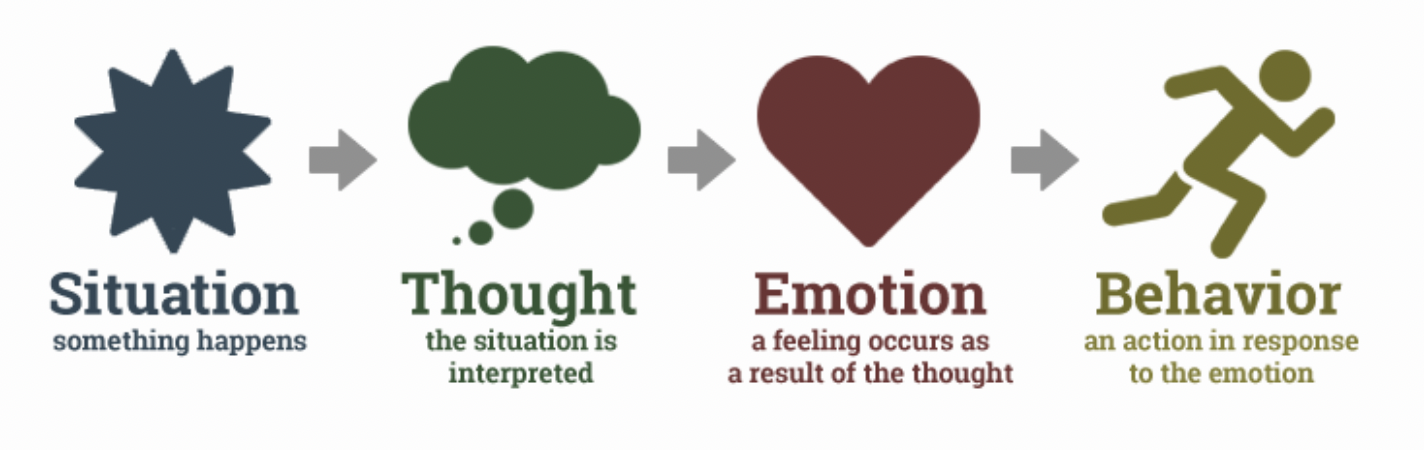
\includegraphics[scale=0.5]{images/cognitive-model.png}
    \caption{This image shows the cognitive model framework that CBT is based around \citep{therapist_aid_psychoeducation}.}
    \label{fig: CognitiveModel}
    \end{centering}
\end{figure}

From the research into Cognitive Behavioural Therapy it can be seen that the techniques used to encourage deeper and more meaningful reflections from patients to provide them new and alternative stratigies to handle situations that will benefit the in the future, are similar to the techniques that have been discussed to encourage reflections in learners about their graduate attributes to analyse how they can develop and improve these skills to benefit them in their future careers and improve their employability.

To examine whether employing a CBT framework into the mobile application will benefit users and encourage them to go through further stages of reflection, an experiment was carried out to compare the results of users who were asked reflective interview style questions, to users who were asked CBT modelled questions. The results of this experiment can be seen in chapter \ref{ExploratoryStudy}.

\section{Existing Products}

Similar existing products were researched and examined before the start of this project.

\subsection{Mahara - University of Glasgow}

University of Glasgow's site Mahara, \citep{mahara_dashboard}, was created to allow students to have a space to create a portfolio, and to create a habit of reflecting on the skills they have developed throughout their time at university \citep{glasgow_university_attributes}.

\textbf{Advantages}
\begin{itemize}
    \item Users are able to make a page about anything, there is no requirement for their posts to be about their graduate attributes and so this provides 
    a level of freedom to users.
    \item It is a social blog website, allowing users to share their blog posts to their friends and tutors. Students are also able to join groups, creating 
    more of a community atmosphere.
    \item The posts are freeform, they can be written text, audio, or video and include attachments and photos. 
    \item Users can choose to have their pages and posts set to private, giving users more control over their content.
\end{itemize}

\textbf{Disadvantages}
\begin{itemize}
    \item This site is not widely known about to students, or students choose not to use it as there are very few users who have any pages or posts. There is
    no developed community on the site.
    \item The site is difficult to navigate, there are 'pages' and 'artefacts' but it is not clear how these are intended to be used, even after reading the 
    description of the site. 
    \item The site has a very basic and minimalist design, which can be an advantage but in this case it does not provide enough content to provide value
    to potential users, as it does not encourage interest in the site.
    \item Although users have freedom to create posts about any topic, this can also be a detriment to the site, as found in the study by 
    \citet{mcdermott_developing_nodate}, as it can lead to student not using the site for it's intended use and lead to less reflections about students graduate 
    attributes.
    \item The site also does not provide the students with any guiding framework with which they can reflect on their learning, making it difficult for students
    to understand what to write.
\end{itemize}

\textbf{Overall} this site has the potential to be used by students as a social blog about their learning and development throughout their time at university,
however, there is a lack of novel and interesting design features and guidance to incentivise users to return to the website to make continuous reflections.
This removes the benefit to the site being a shareable and social blog as there are rarely any other users utilising the features it has. Therefore it has
limited use and is not ideal to encourage users to capture their reflections.

\subsection{Reflectly}

Reflectly is an application intended to capture users reflections on their daily lives in order to improve their mental health and wellbeing, through self-care
and mindfulness. It makes use of positive psychology and cognitive behavioral therapy (CBT) \citep{reflectly_app}. 
A unique component of the Reflectly app is the use of artificial intelligence to gives users personalised questions and trends based on previous entries made.
Although not designed to capture reflections on graduate attributes or learning, there are techniques and design features that are useful to analyse why this
application is popular and enjoyable to use. 

\textbf{Advantages}
\begin{itemize}
    \item Allows reminders to be set to encourage users to reflect regularly.
    \item The app asks users aimed questions, for example "How can you reframe your worries?", this is helpful to users in understanding how to reflect effectively
    and provides a scaffolding to support the user in their mental health development.
    \item Users are able to create different formats of note, the can create a written 'mood check-in', a voice recording, or a photo.
    \item The site uses conversational language to promote a more conversational attitude from the user.
    \item When inputting how a user feels, it asks the user to rate their emotions through a slider scale, meaning that the user does not have to identify
    specific emotions. 
    \item Questions allows users to choose from categories to choose what to reflect on, where they are then able to write down their refelctions freely on 
    this category in a text box.
    \item The voice recording allows users to create a recording on any topic they wish to make, the voice recording provides complete freedom for the user. This
    provides a good alternative to the written reflections where the users must choose a topic to reflect on.
    \item This voice recording capability uses voice recognition to create a written version of the note.
    \item The site provides motivational quotes to uplift users.
    \item The site users enjoyable interface features that make the applications more colourful and interesting to use.
    \item The site provides useful links to resources that may assist the user in their reflections and improving their mental health.
\end{itemize}

\textbf{Disadvantages}
\begin{itemize}
    \item This app requires users to pay for a full subscriptions to be able to use all of the available features that draw people towards using this applciation
    such as the artificial intelligence that will analyse what impacts a users mood. 
    \item When users are carrying out a mood check-in, there is no scaffolding to support the user on how to understand the reasons they could be feeling 
    this way about the chosen subjects. This could make reflection difficult for users to carry out once they have chosen their desired topic.
    \item The voice recording capability converts voice recorded notes into written format, this does not allow the user to listen back to any recordings they 
    have made and instead only keeps the written version. This could be inconvenient if a user would prefer to listen to their reflections and limits customisability.
\end{itemize}

\textbf{Overall} the application is a useful starting point for design for the applications to capture reflections on graduate attributes. However, this app
does not provide a framework to assist users in creating their own reflections, and so further improvements could be made to direct users on the path
of each stage of reflection to ensure they are creating refelctions that will develop their ability to reflect, and therefore in the case of graduate attributes,
allow them to learn and develop these 'soft' skills. Some features would
be useful to implement in the project application, however, many of these features, such as the use of artificial intellgence to analyse trends in users
entries, is not feasible within the scope of the project.

%==================================================================================================================================
\chapter{Exploratory Study} \label{ExploratoryStudy}

Through research into the development of graduate attributes and reflection, similarities were drawn between the practices of reflection to develop and learn graduate attributes, and the practices of Cognitive Behavioural Therapy (CBT) to create healthier and alternative ways to perceive a situation. Specifically the stages of reflection closely match the steps in the cognitive model. 

CBT could have several areas of application to assist students with their reflections on graduate attributes. CBT asks patients to reflect on previous experiences and to analyse their emotions and thoughts during this experience, in order to become more aware of automatic negative thought patterns. Similarly, for students to be able to reflect effectively on their graduate attributes they must analyse situations where they have exercised these skills in the past to become more aware of when they are using them and enabling 'reflection in action'. The questions used to provoke these deep reflections could potentially create scaffolding to assist students in creating equally meaningful reflections on both positive and negative experiences to help them develop and grow their graduate attributes.

CBT involves cognitive restructuring and reframing. This creates an awareness of negative thought patterns that a person does not realise they are experiencing and reframing them to be more positive. Similarly, graduates will not realise they are using their attributes and therefore will not develop them. If graduates were made more aware of these skills and when they are using them then there is more oppurtunity to develop them. Furthermore, in any future situations they will be better equipped to understand the skills they require to benefit their work and environment, and will be equipped to reframe the situation to be more positive and reflective.

Similarly to how \citet{bruno_reflective_2018} stated that learners who work in a reflective environment develop a stronger degree of self-efficacy, people who undergo CBT treatment are able to restructure their core beliefs that impact how they view situations and develop a stronger sense of self-confidence. Employing these CBT techniques could have a similar impact on students and further increase their self-efficacy, restructuring their thinking process to utilise their skills in any given situation. 

Two important components of CBT are journalling and thought records, and activity scheduling and behaviour activation. Journalling allows the user to record their reflections, thoughts and feelings, allowing patterns and tendencies to be identified and adapted \citep{ackerman_cbt_2017}. This will be the fundamental concept employed into the mobile application as it requires the user to take note of all of their reflections. Activity scheduling involves a participant noting something down in their calander that gives them anxiety as it removes the decison making process and creates better habits. This technique will be implemented as the application will provide reminders to encourage the users when to reflect, potentially creating a better habit of reflection with the user.

It was therefore hypothesised that employing the techniques and questioning style of CBT could assist users in their reflections about their graduate attributes and lead to deeper reflections, which in turn would lead to a greater development and situational awareness of these skills. To test this hypothesis a case study was carried out.

\section{Experiment explanation}

Using an A/B testing design a case study was conducted in which a control group received job interview style questions, and the experimental group received questions using the CBT framework. 

The control group was given interview style questions, as these lack any framework or guidance to support a persons reflection. However, this style of questions is still intended to be stimulating enough to encourage a meaningful reflection on previous experiences, to highlight where and when skills have been shown by the interviewee. These questions would be a useful comparison as they simply ask the participant to reflect on the spot, whereas the experimental group is offered CBT scaffolding to support and lead their reflection, potentially encouraging deeper insight, and so therefore any differences this group has are able to be concluded as a result of the scaffolding provided. 

The participants were a convenience sample of 10 students from the University of Glasgow. 5 participants identified as male, and 5 participants idenitfied as female. These 10 participants were randomly assigned to one of the groups, either control or experiment group.

After giving consent to take part in the experiment, participants were then directed to the corresponding Google Form which either asked the participant to reflect with the job interview style questions or the CBT style questions. These surveys can be seen in the appendix (INSERT LINK).


\section{Results}

To analyse the results of the experiment, the stages of reflection stated in section \ref{backgroundReflection} were used. In each of the participants answers, any comment that involved one of the stages of reflection were highlighted in a corresponding colour code. These were then assimilated to show how many participants had engaged with each stage of reflection at least once during the experiment, and placed in a graph to show the comparison of results with and without the use of CBT.

\begin{figure}[h!]
    \begin{centering}
    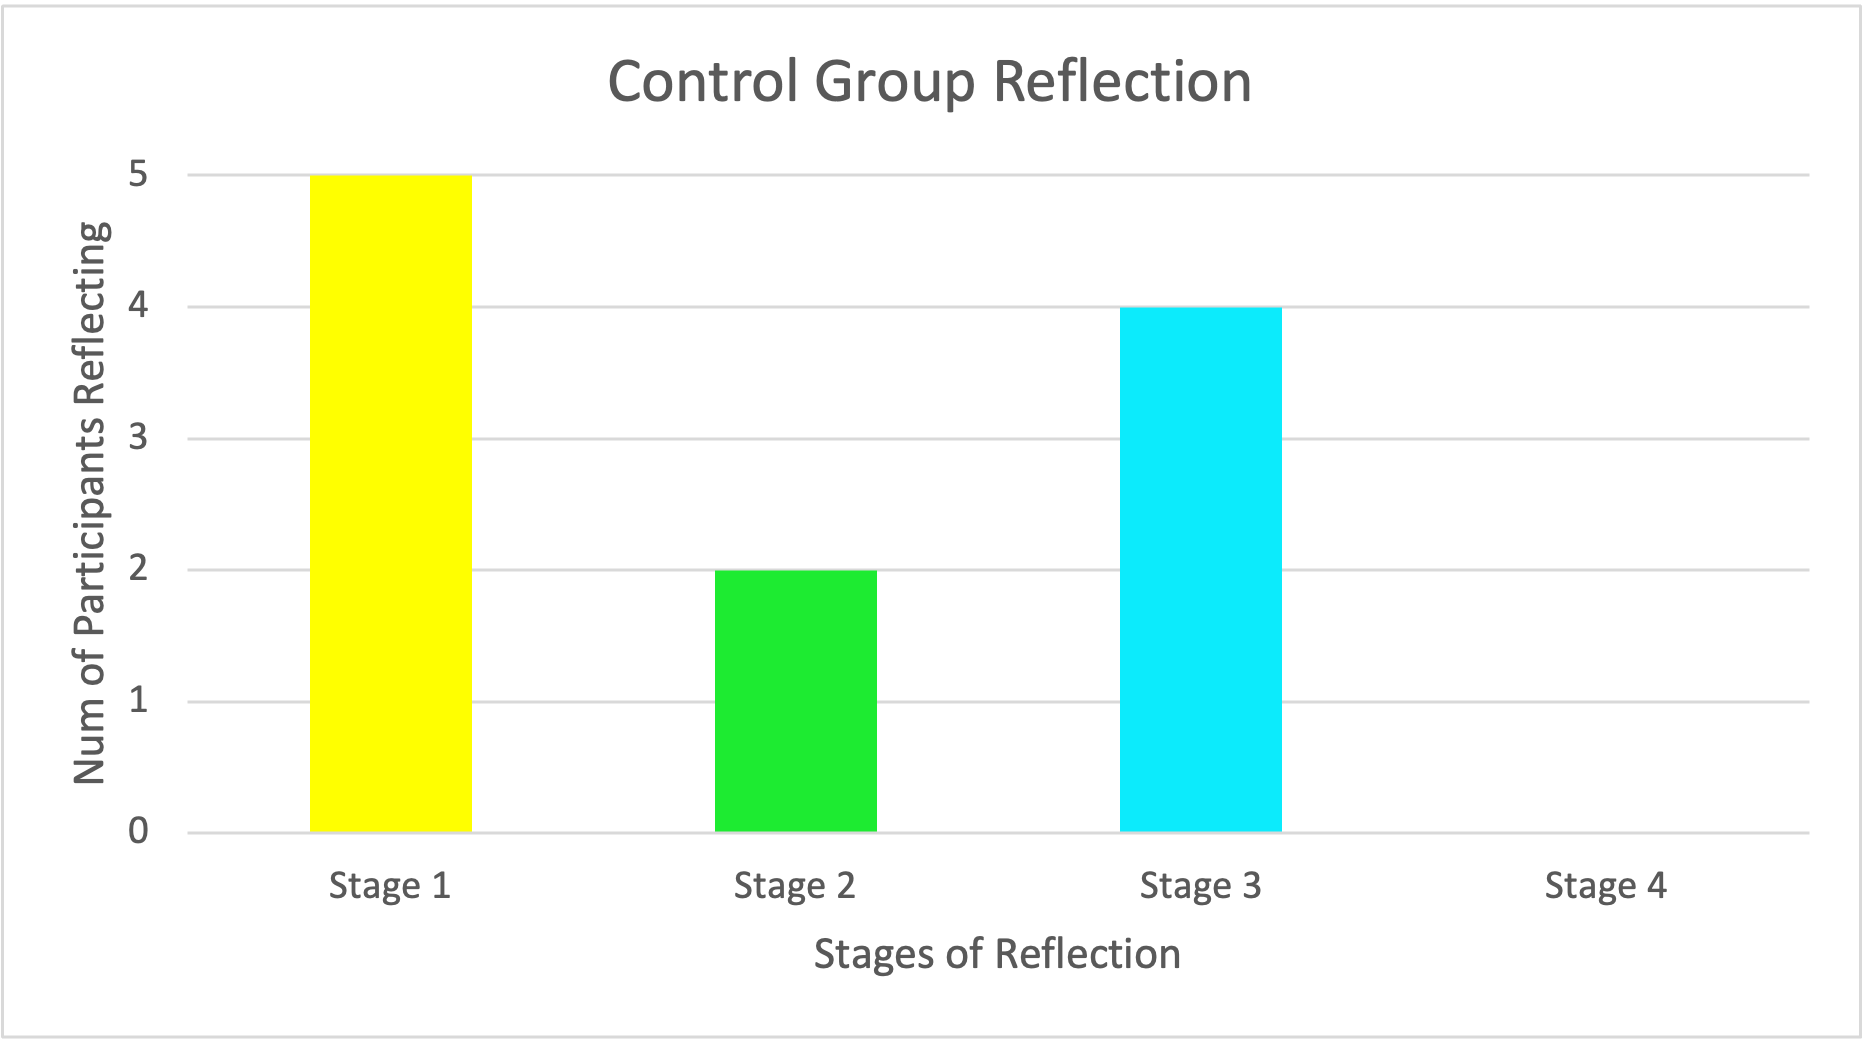
\includegraphics[scale=0.75]{images/ABControlGraph.png}
    \caption{This graph show the number of participants in the control group that carried out each stage of reflection. These participants were not given the Cognitive Behavioural Therapy framework to encourage their reflection. It can be seen that most participants went through the first 3 stages, however, none of the participants carried out the final stage of reflection.}
    \label{fig: ABStudyGraphControl}
    \end{centering}
\end{figure}

\begin{figure}[h!]
    \begin{centering}
    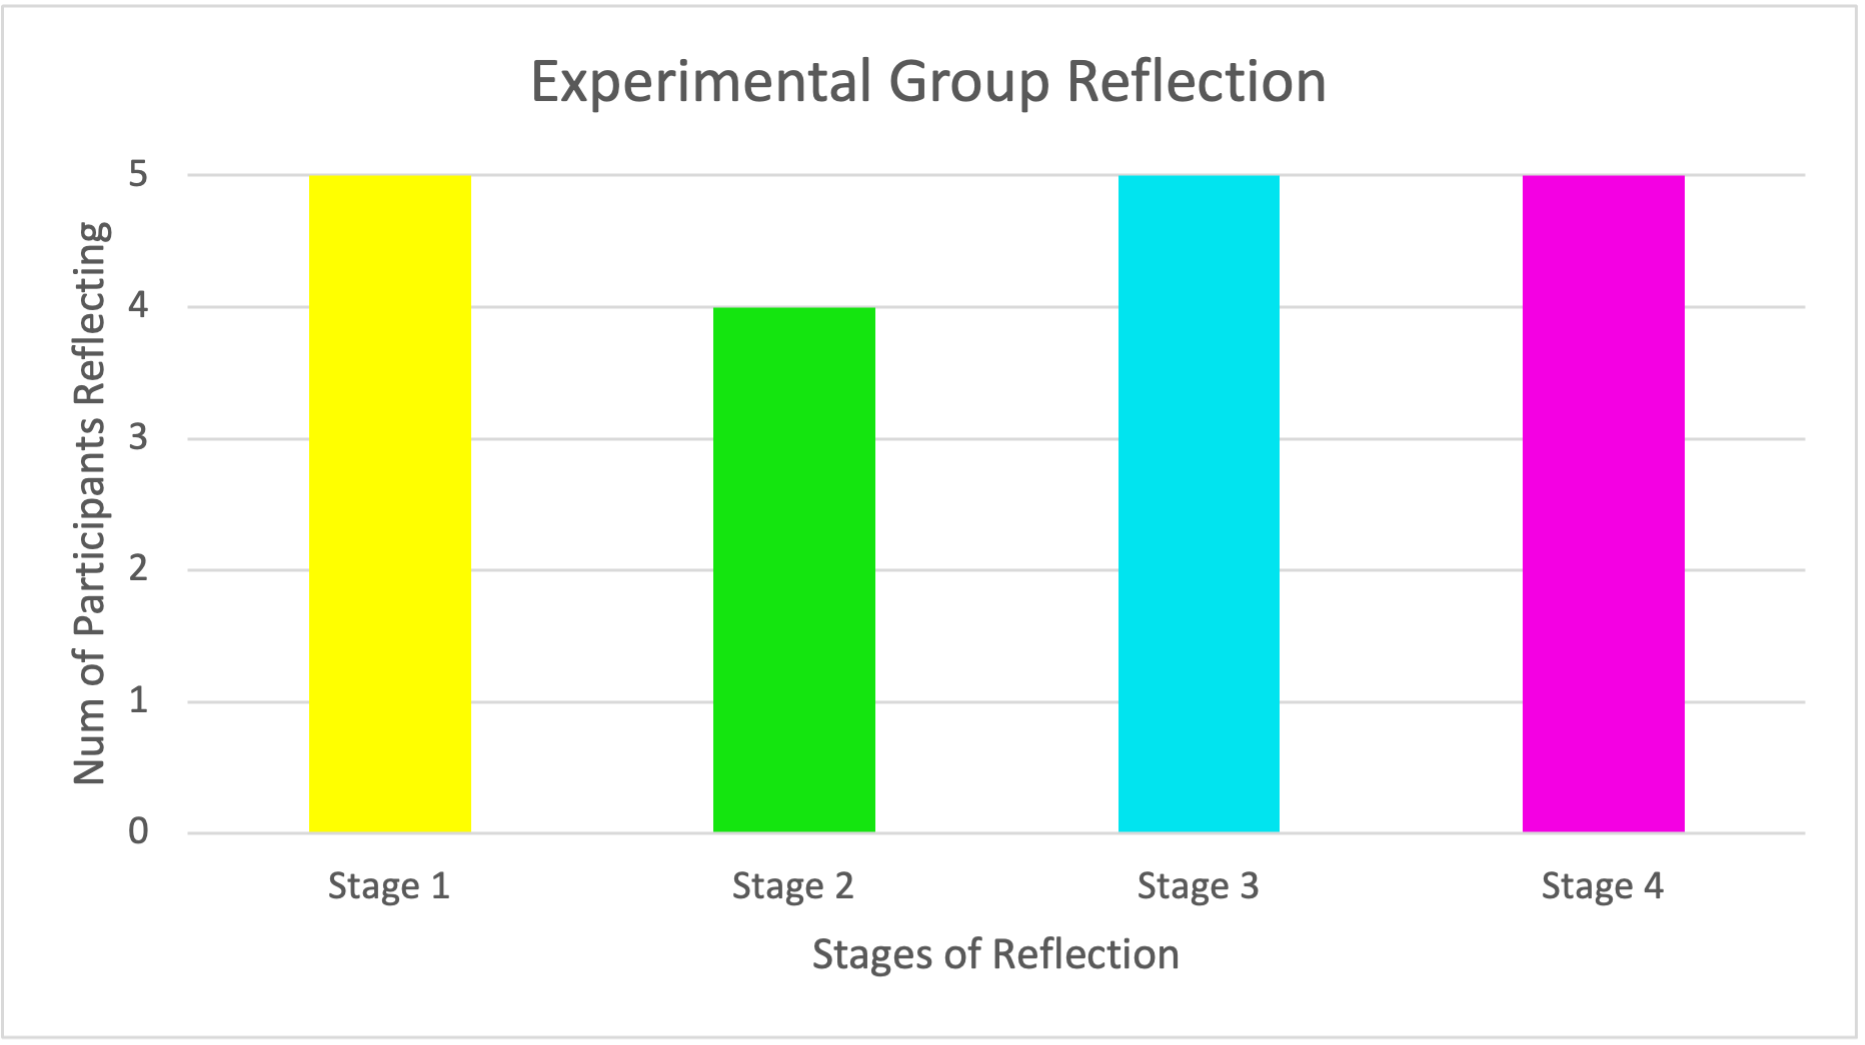
\includegraphics[scale=0.75]{images/ABExperimentGraph.png}
    \caption{This graph show the number of participants in the experimental group that carried out each stage of reflection. These participants were given the Cognitive Behavioural Therapy framework to encourage their reflection. It can be seen that all bar one participant went through every stage of reflection in their answers.}
    \label{fig: ABStudyGraphExperiment}
    \end{centering}
\end{figure}

NEED TO ADD SOME SORT OF P-VALUE ANALYSIS TOO!!!! I DONT THINK I DO ACTUALLY, BUT MAYBE ADD SOMETHING TO GIVE THE RESULTS SOME WEIGHT BUT NOT TOO MUCH WEIGHT???

The results of this experiment showed that the participants given the job interview style questions were able to all carry out the first stage of reflection in which the person simply describes the concrete experience. This was also the case for the experimental group. 

With stage 2 of reflection in which the person describes the emotional state they were in during the experience, only 2 of the participants from the control group went through this stage, compared to 4 of the experimental group.

Stage 3 involved particpants examining the cause and effect of the situation and how their actions and behaviour effected the outcome. 4 out of 5 of the control group reached this level of reflection, whereas all 5 participants in the experimental group reached this stage.

Finally, for stage 4 of reflection in which participants were expected to suggest alternative thoughts and examine the alternative ways the situation could have been handled and whether they gained the best outcome in order to acquire a new perspective and improve in the future, none of the participants in the control group reached this level of reflection, which distinctly contrasts the experimental group in which every participants reached this level of reflection.


There is a significant difference within the results of the control and experimental group. These results clearly show that with the framework provided through CBT techniques, students were better equipped to have deeper and more insightful reflections on their graduate attributes. This CBT framework was able to lead to students through each stage and encourage them to provide more cognitive analysis on the given situation. Futhermore, students in the experimental group had higher word counts for most answers. Although a higher word count does not provide evidence that further reflection is occuring, it can suggest that participants were exploring their thought process further, and taking more time over their answers. 

Due to the representative sample taken of students, this case study can provide further evidence to agree with the statements made by \citet{bruno_reflective_2018} that state that students require clear instructions in order to reflect effectively, which the CBT framework can provide. The casestudy further suggests that CBT can lead to deeper reflections from students, and could be integrated into reflective models students partake in. However, due to this case study being carried out once and the small sample size, these results are not generalisable and further research would need to be carried out. 

\section{Limitations}

Although this experiment was able to prove that the use of CBT techniques and structure encouraged further reflection from students in this case, it cannot provide evidence of the long term effects of this form of reflection could have on students and how it impacts their graduate attributes. 

In future work, participants should be asked to answer these questions on a weekly basis for an extended period of time. Before conducting the experiment users should be asked to fill in questionaires to assess their level of graduate skills and their confidence in reflection. This should then be compared with the answers they provide at the end of the experiment period to examine whether students had increased their level of development of their graduate skills and whether they felt more confident in their ability to reflect. The answers given on a weekly basis should also be examined to identify whether, over time, students were increasing their level of reflection in their answers. 

This would allow conclusive evidence to be given on the benefits that the use of CBT scaffolding could have on students and their graduate attributes. This however, was not within the scope of the project due to time and resource contraints. 


%-------------------------------------------------------------------

%==================================================================================================================================
\chapter{Analysis/Requirements}

This project was presented by a Univeristy of Glasgow lecturer, Dr. Matthew Barr, who required a mobile application to be made to capture reflections on graduate attributes. A list of requirements was created in weekly meetings. This was an agile process where the newest version of the application, experiments, and design documents were presented and discussed each week. Dr Barr's paper "Graduate Skills and Game-Based Learning: Using Video Games for Employability in Higher Education" provided enough detail to gain an understanding of what graduate attributes were and how they were learned \citep{barr_2019}. Lecture notes from the classes Mobile Human-Computer Interaction and Human-Computer Interaction were also used to gain understanding of how to create a usable and satisfying application for users, as well as how to conduct various evaluations and experiments that would be required for this project. Further requirements were gathered through personal heuristic evaluation as the project progressed, this allowed iterative improvements to be made to the application, increasing the overall usability.

\section{Problem Specification}

The main expectations for the application are listed below. The key requirement, as stated in the introduction, was to allow users to capture their reflections on when and where they have used their graduate attributes. It was decided that the best method to acheive this was to allow users to quickly and conveniently reflect using a mobile application. As the application will use Cognitive Behavioural Therapy techniques and prompts to encourage the user to reflect more meaningfully, they can in their own time, deepen their understanding and development of these skills. The ability for users to make reflection easily was tested in the user evaluations later in the project. 

To begin creating the list of functional requirements of the GradReflect app, multiple user scenarios and user stories were initially created for students, interns/apprentices, recent graduates and experienced members in the workplace, these can be seen in appendix (REFERENCE). However, through discussion with Dr Barr, it was decided the main users of this application would be students, and the application should designed as such. The list of functional requirements below describes actions that users should be able to perform with the application. The list of non-functional requirements are requirements of the applications itself. These requirements follow the MoSCoW requirements building format including Must Have (MH), Should Have (SH), Could Have (CH) and Wont Have (WH) \citep{consortium_chapter_2014}. Requirements marked with * were added throughout the project as different iterations introduced possible new functionalities. 

\textbf{Functional requirements}
\begin{itemize}
    \item \textbf{MH} Users must be able to capture a reflection of how and when they have exercised and developed their graduate skills, this can be in either written OR audio form.
    \item \textbf{MH} Users must be able to delete a reflection created, as well as being able to review it at a later date, however users should not be able to update or edit a note after it's creation. 
    \item \textbf{MH} Users must be able to turn on notifications.

    \item \textbf{SH} Users should be able to select a skill from a pre-defined list to avoid mistakes and allow for future potential filtering.
    \item \textbf{SH} When creating a written note, there should be help buttons that explain to the user how they should answer each questions and provide an example, this will give them clear instructions to allow effective reflection.
    \item \textbf{SH} Users should be able to give their note a title to allow for clear representation of what a note contains, and allow for future potential searching or filtering.
    \item \textbf{SH*} Users should be able to create a reflection in BOTH written and audio form. This will allow both structured reflections and freeform spoken reflections for convenience. 
    \item \textbf{SH} The application should contain a description of each of the skills that users are expected to develop and reflect on during the use of the app. 
    \item \textbf{SH*} Users should be able to search for the name of a note or a skill category to filter the notes in the list by skill.
    \item \textbf{SH} The application should have a Settings page to view information about the application.
    \item \textbf{SH} GradReflect should have an About Page within the settings that tells the user how to use the app correctly to make reflections, giving further clear instructions to the user. 
    \item \textbf{SH*} Users should be able to view statistics based on the reflections written into the application.
    
    \item \textbf{CH} The application could implement Cognitive Behavioural Therapy techniques to aid the reflection and provide users with a suitable framework to support them and provide clear instructions on how to reflect. 
    \item \textbf{CH*} Users could have the ability to customise their experience of GradReflect and have the ability to switch between dark and light themed interface.
    \item \textbf{CH} GradReflect could have links in the Settings page that take users to useful pages related to the app and graduate attributes to provide further insight and education on graduate attributes.
    
    \item \textbf{WH} It was decided that users will not be able to upload reflections onto Moodle as this is not within the scope and does not provide enough benefit to users in completing the aims discussed in Section \ref{IntroAims}.
\end{itemize}

\textbf{Non-functional requirements}
\begin{itemize}
    \item \textbf{MH} Must be intuitive and easy to use. An application that is easier for new users is more likely to encourage them to continue to use the application and have an interest in it.
    \item \textbf{MH} Must help users to to create meaningful reflections about their graduate skills. The ability for the users to reach more of the stages of reflection will help to develop these skills within students.
    \item \textbf{SH} Users should be able to create quick reflections.
    \item \textbf{SH} The application should be able to encourage the users to want to continue using the application in the future.
    \item \textbf{SH} Users should find the features of the application useful and find the value in using an application like this to reflect. 
\end{itemize}


\section{Chosen Limitations}

Due to this application being designed and created for iOS devices, users will not be able to download this application onto their own devices without the application being uploaded to the Apple app store. This was not possible as this would require a paid Apple developer license and is therefore outwith the scope of this project. However, due to this it meant that some limitations were chosen to create more of a prototype of the application to test and evaluate the value of an application for capturing graduates attributes, that in the future could be taken onto other platforms and for general use by the public.

Reminders will not be able to be set by the user, instead they will turn on the notifications and a notification will fire after 10 seconds. This was decided for ease of testing. The response time of notifications was therefore immediate and as the application will be run on a simulator that is not always running, users and testers will not be able to use GradReflect for extended periods of time that would allow a notification to be set in the future. In future developments of this application, users would be able to turn on notifications and the notifications would remind the user to reflect once a week on their chosen day. 

\section{Changes to the Specification}

The specification was changed in discussion with the project supervisor as described at the beginning of this chapter, as well as due to time contraints and research paths that opened up during these conversations. The main change to the original specification given was to integrate the use of Cognitive Behavioural Therapy techniques into the application. This was chosen during research into reflection and situations where people have had to reflect deeply and meaningfully about their real-life experiences. This was taken as a research question into the project to evaluate its possible benefits in aiding the reflection of users about their graduate attributes. 

Each possible feature of the application was also evaluated based on the time it was likely to take as well as its usefulness. As a result, the decision was made to remove the ability for users to upload their reflections to Moodle. This was due to the research direction taken with the use of CBT questioning. The encouragement of users to include their thoughts and feelings into their reflections of the app caused it to be more personal than users would perhaps feel 
comfortable uploading onto Moodle. Upon conversation with peers it was also noted that students would be unlikely to use this feature and would rather just have these reflections on their personal devices. The decision was then taken to include a link to Moodle on the Useful Links section of the mobile application instead, to still maintain a connection with the university and the application. 


%==================================================================================================================================
\chapter{Design}

This chapter will discuss the design of the product, starting with the design of the CBT modelled questions. The user interface design will also be discussed including the reasoning behind a number of key design decisions which were made in order to meet the requirements laid out in the previous chapter. Finally, the chapter will go on to examine the tools and technologies that were used for the project. 

\section{Encouraging Reflection}

In order to encourage reflection, various use cases and features were designed to give users more reasons to use the application.

\subsection{Written Notes}

Written notes were required to give users the oppurtunity to reflect using the CBT methods described in chapter \ref{Background}. The questions would be designed similarly to the questions used in the experiment described in chapter \ref{ExploratoryStudy}, with only minor alterations to allow more functionality within the application. 

Each question was required to be stated clearly and consisely, giving users the availablity of a helper button to give more insight into how the user can answer this question and an example given. This will allow the user to understand what the application is expecting of them and further encourage deep and meaningful reflections as they have been given the required instructions needed to do this \citep{bruno_reflective_2018}. (ADD APPENDIX REFERENCE TO THE APP QUESTIONS AND PROMPTS THAT WERE USED)

The question asking about emotional reaction was chosen to be a sliding scale from a clear negative reaction to a positive reaction. This means that users are not required to choose an emotional reaction, which can at times be difficult to identify, instead they are given an easier option of gauging how postively they felt. 

Users were also given the oppurtunity to be able to click on previously made notes to review, reflect on, and delete these previous entries, however, they were not able to edit or update any of their reflections. This was decided to mirror the CBT behaviours of writing down reflections in a journal where they cannot be altered posthumously. This would stop users from using hindsight on their previous experiences and gain an accurate representation of their experiences during that time. 

\subsection{Recorded Notes}

Users were provided the option of creating a note through a voice recording. This would add further convenience to quickly reflect or record an experience that they may want to return to later to further reflect on. There is no framework provided when creating a recorded note to allow users the freedom to reflect however they want, the ability to say what is on their mind without any framework can be easier as it is often easier to speak freely than to arrange ones thoughts into a cohesive written sentence. 

Users are able to record, delete and playback a recording with and without a title provided by the user. 

\subsection{Statistics}

Statistics on a users written reflections were also included. This was created to allow users insight into their own reflections, focussing their development of skills. It provides detail on both data organsied by skill and over all of the notes taken. The user is able to view how many notes they had made overall and the average words per note. They can also scroll through each skill to see how many notes they had written, their average words per note for that skill and their average emotional response for that skill. 

These useful insights will allow the user to see both their strengths, through the skills with a high number of notes, and their weaknesses, through skills with a comparitively low number of notes. This will focus their goals showing where further development is required. It will also show users where they need to potentially reflect deeper thorugh the word count. If the word count is low it is likely they not spending enough time reflecting, or reflecting in enough detail. And lastly, they will gain insight into how they feel about certain skills, if their average emotional response to a skill is low then they can evaluate why they feel this way about this skill and potentially attempt to develop this skill further.

\subsection{Additional Assistance}

Additonal assistance to reflection was also designed in the homepage and the settings page. Upon entering the application users should be greeted with descriptions of each skills and an example of where it could be used. Clear descriptions and instructions of the skills will increase a users awareness of these skills in their everyday life, helping to develop them. 

Further descriptions of how to use the application are given within the settings page, further increasing the level of clear instructions needed to help students be able to reflect effectively \citep{bruno_reflective_2018}.

\section{User Interface}

The user interface was designed to help users quickly learn how to use the application and start reflecting. To do this it was required that the interface was intuitive and easy to use, this would be made possible through an attractive and straightforward design. This section describes some of the techniques used during that design process.

\subsection{Initial Prototyping}

In order to gain insight into what each page would require and ensure all features had been considered, all designs went through a prototyping process. 

Design of existing note taking applications were considered so that new users to GradReflect could still find the interface familar. Some of these similarities are listed below.

\begin{itemize}
    \item Title of the view stated in bold at the top of the view.
    \item A search feature at the top of the view.
    \item Notes in a listed format with a title and date created displayed.
    \item A return button at the top left corner of the view.
    \item An edit button, or swiping functionality on a specific note, to delete notes.
    \item Recordings page with a large recording symbol at the bottom of the screen.
    \item A settings page containing the creation details, customisation of the application and further information about the application.
    \item TabViews containing informations or images that users can scroll through, containing small dots at the bottom to show which tab the user is on.
\end{itemize}

Some of the applications studied for this were: Apple's Voice Memos \citep{apple_inc_voice_2021}, Apple's Notes \citep{apple_inc_notes_2021}, Google's Keep Notes \citep{google_llc_google_2021} and Collateral \citep{vargas_collateral_2021}.

Taking inspiration from existing applications was decided as a good starting point as external consistency allows users to feel more comfortable and understand the application better when it is similar to what they have used in the past \citep{schlatter_visual_2013}. This helps to satisfy the requirement that the application be easy to use. 

Figure \ref{fig:PaperWireframe1} shows the initial prototype developed for GradReflect. A homepage design that directed users to each section of the page was first envisioned. This homepage could provide users with descriptions of each skill and how to use the application. Initially, it was considered to have the skills only appear on a users first time using the application, and then would be held within the settings section of the application following this, however this idea was discarded instead for the skills being always available on the home page to scroll through. This would help users instantly understand what to do when first opening the application, but if users have used the application several times they are able to head quickly to the section they wish to use, whilst also having the easy availability of the skill descriptions if users want to refresh their knowledge. 

Paper prototypes were created for the rest of the views of the application in a similar way to the homepage, as seen in figure \ref{fig:PaperPrototypes}. This protyping stage was extremely valuable and assisted in speeding up the implementation stage as the design decisions had already been carried out, giving a clear idea of how the final product should appear, ensuring the requirements would be met. However, some alterations from these designs were made for the final implementation.

These designs were then implemented into high fidelity wireframe prototypes, using iOS design features, which can be seen in the appendix section (ADD APPENDIX REF).

\begin{figure}
    \centering
    \begin{subfigure}[b]{1\textwidth}
        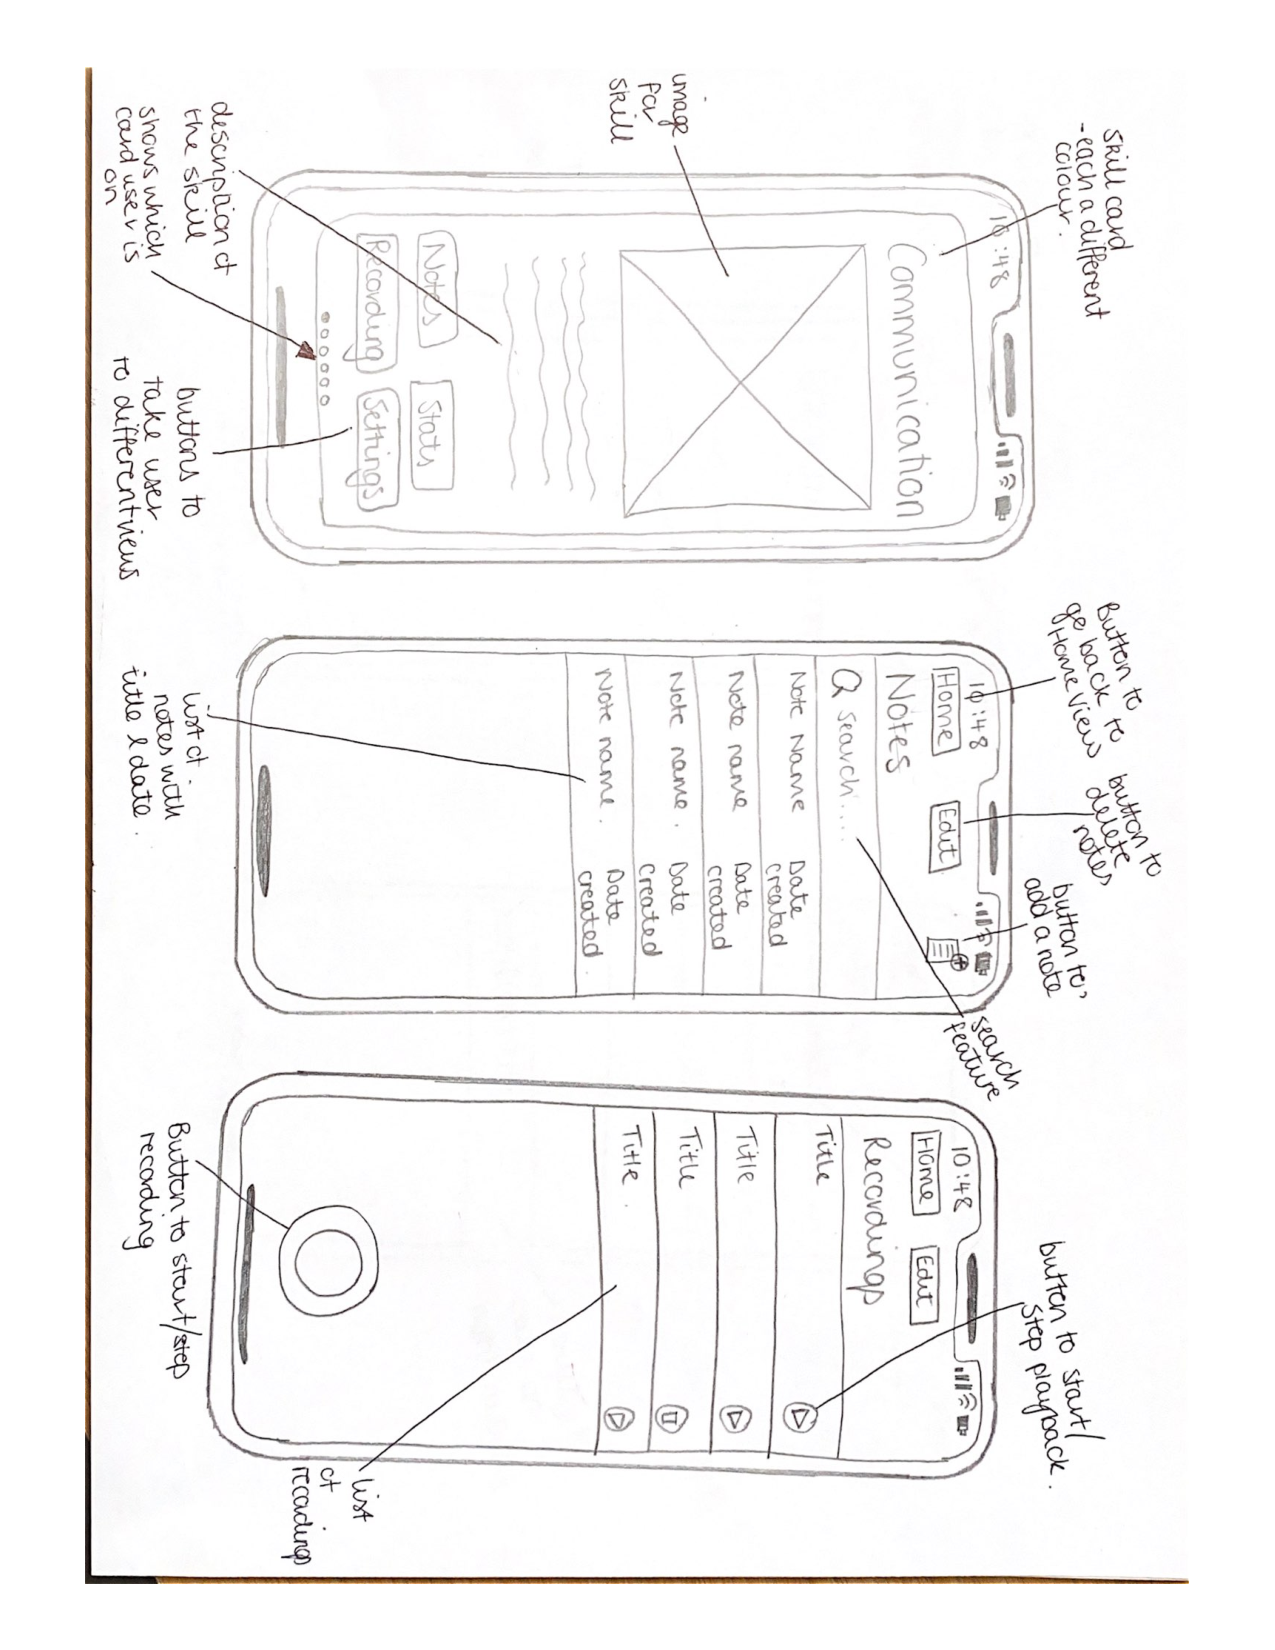
\includegraphics[scale=0.45, angle = 90]{images/PaperWireframes1.pdf}
        \caption{Initial paper prototype designs for the Home, Note and Recordings views.}
        \label{fig:PaperWireframe1}
    \end{subfigure}
    \begin{subfigure}[b]{1\textwidth}
        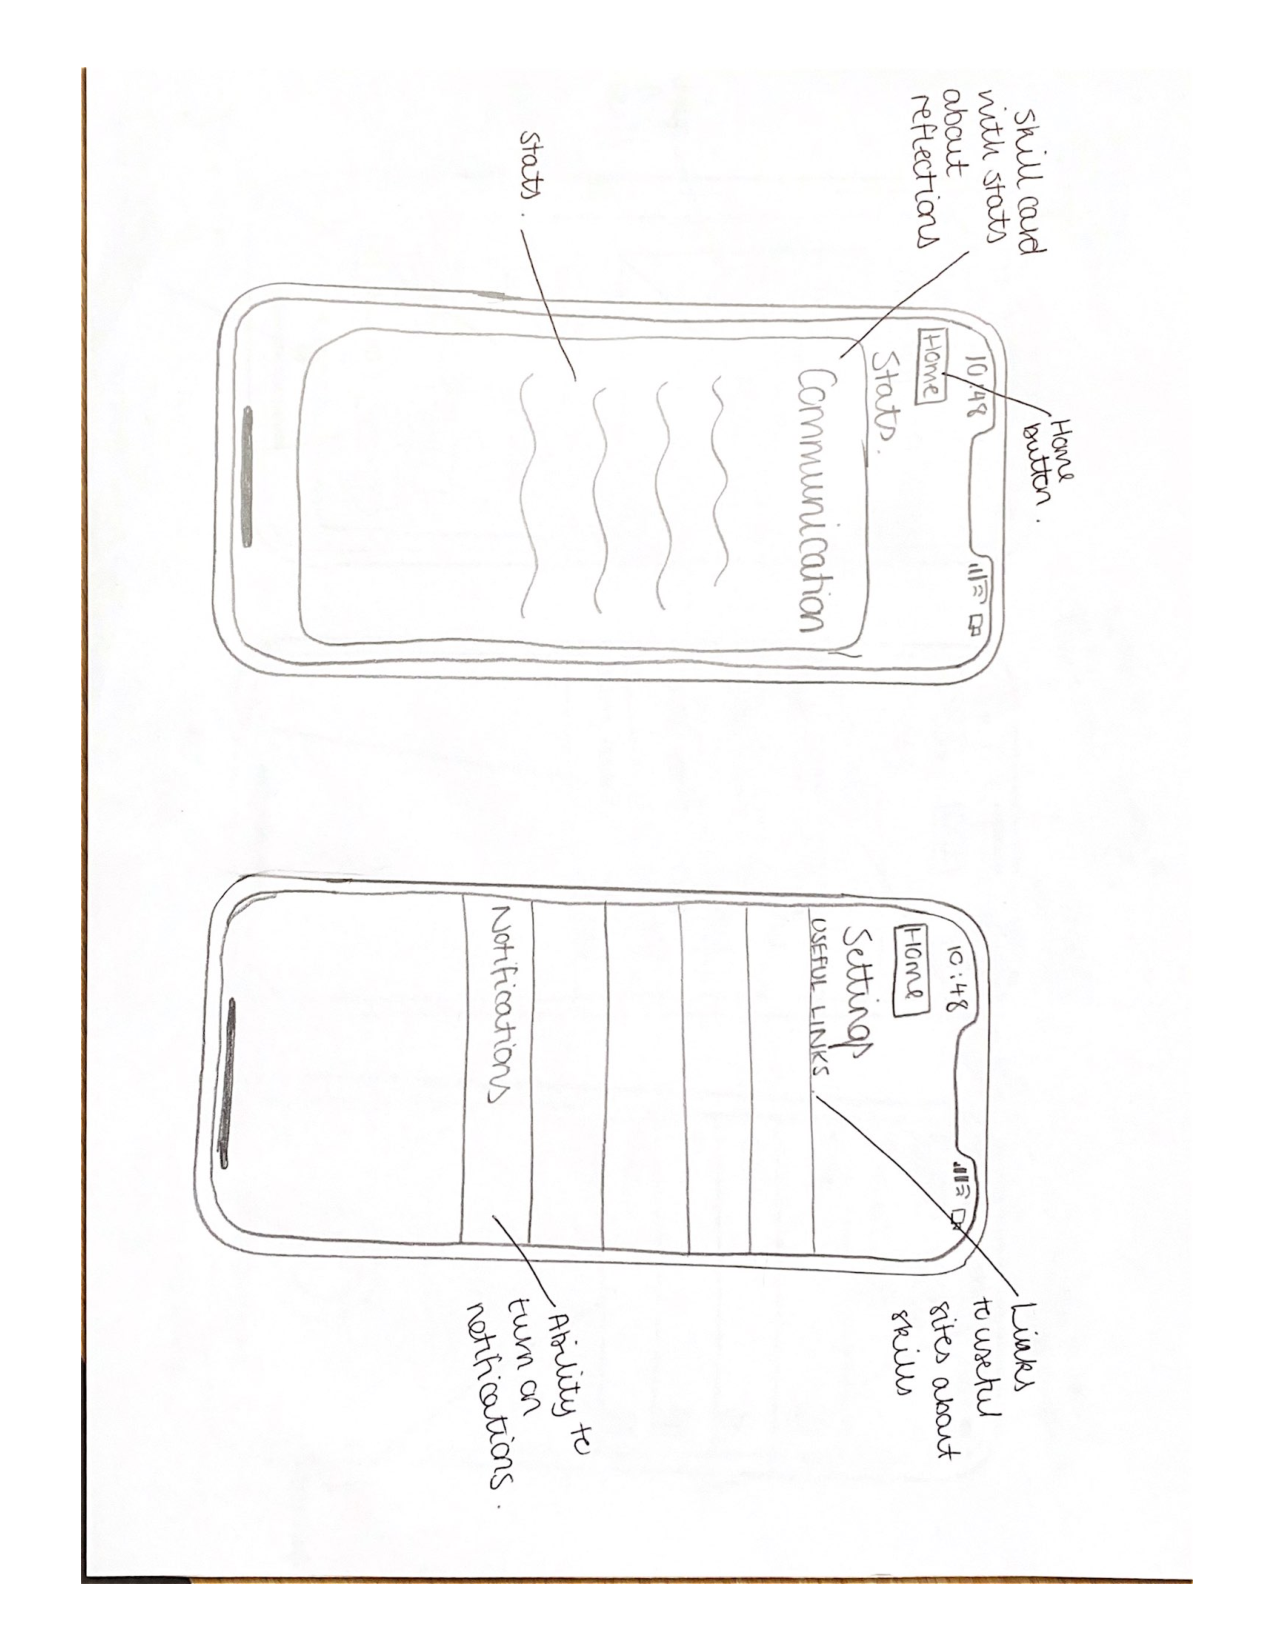
\includegraphics[scale=0.45, angle = 90]{images/PaperWireframes2.pdf}
        \caption{Initial paper prototypes for the Statistics and Settings view.}
        \label{fig:PaperWireframe2}
    \end{subfigure}     
    \caption{Scanned files showing the paper prototypes that were made in the early stages of design, iterative changes were made to design following these protptypes for the final product.}
    \label{fig:PaperPrototypes}
\end{figure}

\section{Technologies}
Time was taken at the beginning of this project to choose appropriate technologies. The technologies used and the reasons behind those choices are described here.

\subsection{iOS Mobile Application}

A mobile applications was chosen as the goal of the application was for users to create, save and review thier reflections on graduate attributes and did not require user accounts or external information sharing that is made easier by using web frameworks. It was also due to the personal nature of the reflections being carried out by users and the use of CBT. The ability to carry out these reflections on their phone can lead to more intimate and personal reflections from users, as it is held on the users personal device instead of on an online account or on their desktop. Additionally, as these reflections are on personal experiences, it is convenient for the user to be able to carry out reflection on-the-go on their mobile device. This allows the user to be able to instantly reflect on a situation and capture more accurate depictions of events and their thoughts and emotions. 

It was also decided to create this app using iOS development due to the appealing interface design associated with Apple applications, benefiting usability. iOS was also chosen due to it's familiarity and known interface design concepts.

\subsection{iOS Development}

Although Apple keeps iOS development exclusive to other Apple devices, making it difficult for an aspiring iOS developer using another operating system, there are useful advantages to creating an application using Apple developement. Creating an iOS application for any platform, Mac, iPhone, iPad, Apple Watch, or Apple TV, requires the Apple \textbf{XCode IDE}. 

\textbf{Swift} is the language used to create mobile iOS applications. It is a a modern language with inferred types making it less prone to mistakes, and syntax that encourages clean and concise coding. This syntax can appear to be strict at times, but allows for the safeguarding and prevention of errors, improving readability with its similarity to natural english \citep{altexsoft_swift_2021}. This allows for easier learning of the language and an easier start to development.

\textbf{SwiftUI} was chosen for the interface lifecycle. SwiftUI is a new and innovative way to create interfaces that can allow for entire applications and their functionality to be written using it \citep{apple_developer_xcode_2021}. It uses declarative syntax to allow a developer to simply state what they want the interface to do. A key benefit to using SwiftUI is the preview editor that ajoins the code editor, displaying the app with any device and orientation. As code is written it is instantly complied and the preview shows the changes live. This allows the developer to run the current view of the app and interact with the UI elements, giving a clear indication to the developer of how the interface looks and works, and allowing for debugging and editing \citep{apple_swiftui_2021}. These benefits allow for easier creation of the applications interface and it's functionality, and assist in creating a more visually appealing and simple interface that will be easier for users to utilise.



%==================================================================================================================================
\chapter{Implementation} \label{implementation}

This chapter describes the steps taken to implement GradReflect, described in previous chapters, and the technical descisions that were made during this process.

\section{User Interface}

The user interface was implemented using SwiftUI with an aim to make it easy to use and visually appealing. 

\subsection{Model View ViewModel}

SwiftUI presents both useful features and challenges when creating an application. Instead of a typical Model View Controller design pattern, SwiftUI is state-driven and declarative, implementing a Model View ViewModel design pattern built into the framework \citep{naumov_swiftui_architecture_2019}. Tutorials from CodeWithChris \citep{ching_codewithchris_2021}, SwiftUI Masterclass Course \citep{petras_swiftui_2021} and Blckbirds \citep{blckbirds_learn_2021} were used to learn the basics of SwiftUI development and begin implementation.

\textbf{Model:} The model classes within SwiftUI are used as a data container that define a structure that will be written to and fetched from. An example of this is the Skill Model. This defines that each skill contains an id, a title, description, an image, and gradientColours with defines the colour scheme for that skill card. This model is also reused for the Statistics view.

A model is also created to hold the note entries created by the user via CoreData, the permanent storage organising the data in an entity-attribute relationship. Core Data involved a steep learning curve, however, proved to be beneficial due to the ability to manipulate the data within the fetch request in a single line of code, and it's ability to track changes through the persistant storage. This made for greater simplicity whilst implementing. CoreData is saved using an NSManagedObject which uses optimised storage and retrieval methods with key-value coding and observing, this is faster than other means of storage and retrieval, including get/set methods \citep{apple_developer_documentation_core_2021}. CoreData entry is operated on via the ViewModel, translating user events received from the view into CRUD (create, read, update, and delete) operations that can change the model and its data. The flow of data can be seen in figure \ref{fig:MVVMDataFlow}. 

\textbf{View:} The view is responsible for displaying the UI and animations. A secondary responsibility of the view is to receive any user interactions and pass these to a view model for interpretation \citep{bulavin_modern_2020}. The view is made up of views and controls, each view represents a building block of user interface. The controls allow the user to interact with this interface. SwiftUI made it easy to build a UI, allowing the standard building blocks to be altered to fit the needs of the project concisely and simply, making this aspect of implementation quick.

\textbf{ViewModel:} The ViewModel is responsible for dictating how data should be represented in the view, as well as interpreting user inputs into actions and updating the UI state and behaviour accordingly. The ViewModel can take form of the @State variables bound to the view, updating the UI anytime changes are made to the state. These ViewModels can also take the form of a distinct ObservableObject class. As an example the Router class is a ObservableObject class, this handles when a view's StateObject 'current page' variable will change, and update the view to show the requested page. 

\begin{figure}
    \centering
    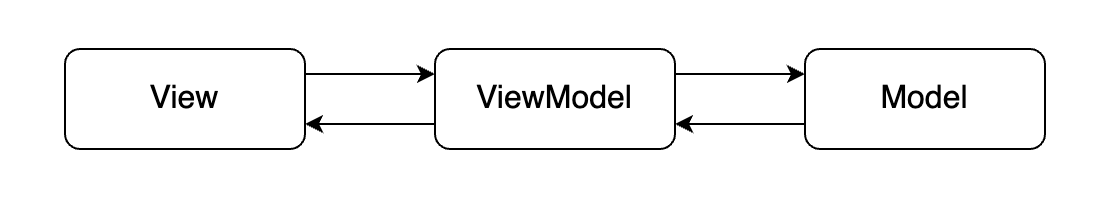
\includegraphics[scale=0.5]{images/MVVMDataFlow.png}    
    \caption{This diagram shows the data flow between components in the Model View ViewModel (MVVM) design pattern 
    \citep{bulavin_modern_2020}.}
    \label{fig:MVVMDataFlow} 
\end{figure}


\section{Aesthetics}

\subsection{OS native appearance}

SwiftUI enforces a standard design of common on-screen objects. These were found to be very user-friendly and attractive, with only a minor issue highlighted in the usability study in section \ref{evaluation}, where users attempted to delete a note within the review, instead of using the edit button on their first attempt. Another advantage of the SwiftUI framework is that it allows for the creation of existing iOS features, such as the Edit button, to give a cohesive and familiar appearance on iOS phones. This was beneficial as it meant that there were pre-built buttons with pre-written functionality. However, it also meant that this code was not able to be altered to adjust functionality. Despite this, it was beneficial as it gave the interface a familiar look and features, improving usability. It also allowed the project to focus on the problems specific to the aims of the project, instead of the detailed aspects of the design. The user interfaces for the main views of the application can be seen in figure \ref{fig:appMainViews}

\begin{figure}
    \centering
    \begin{subfigure}[b]{0.3\textwidth}
        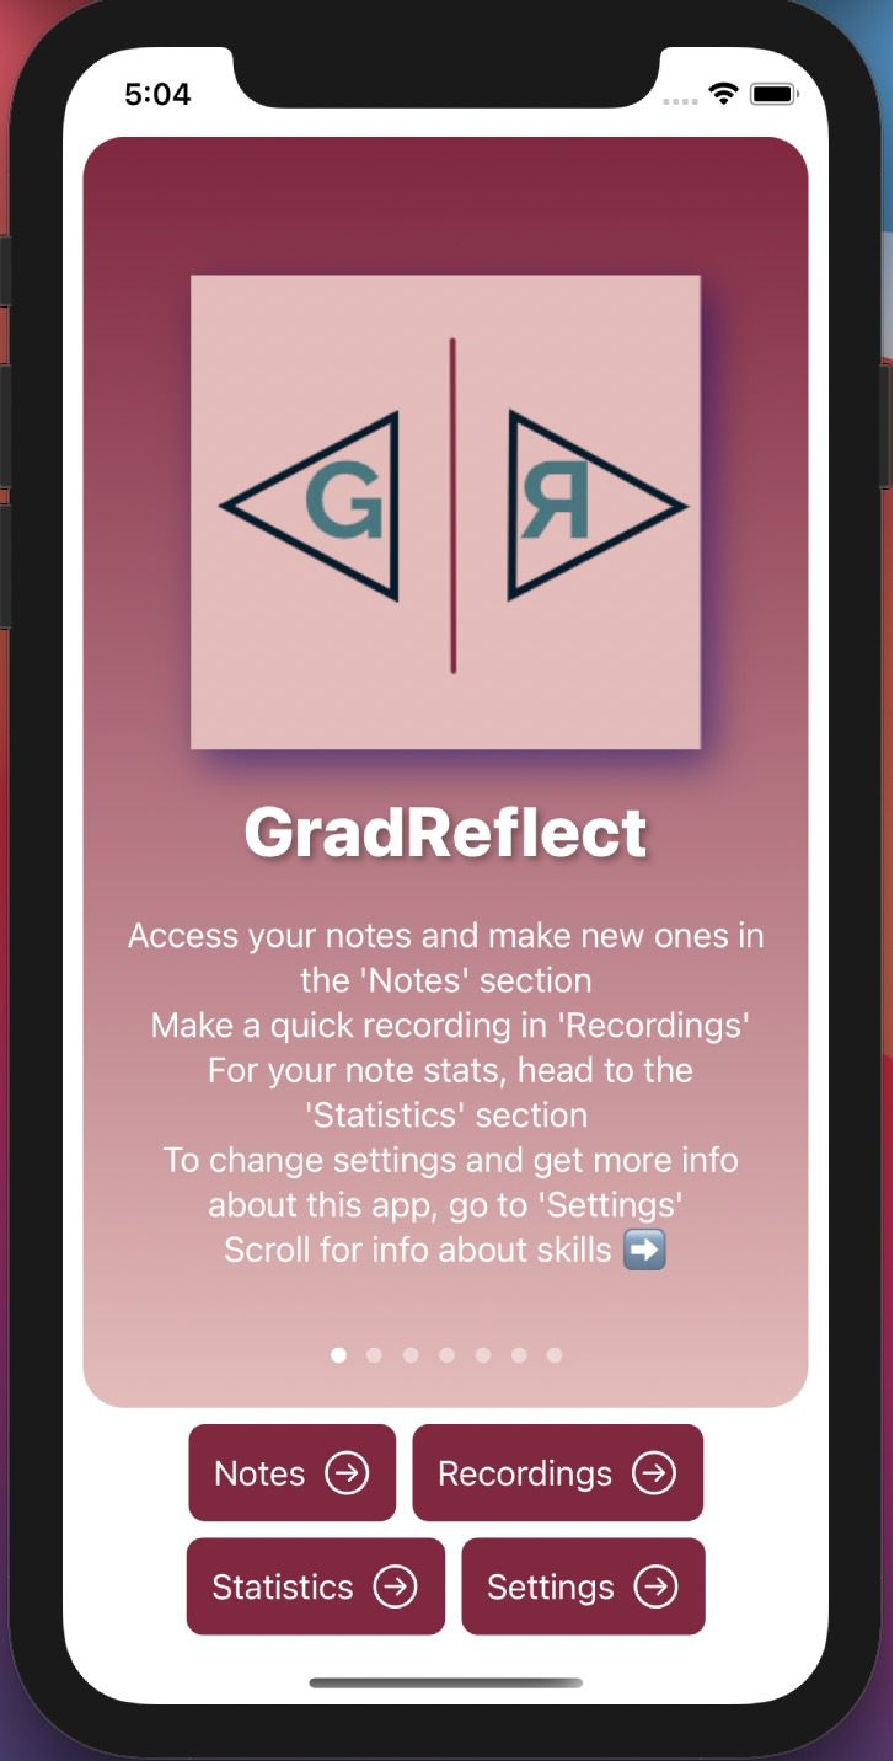
\includegraphics[scale=0.25]{images/appHomeScreen.pdf}
        \caption{Home view}
        \label{fig:appHomeScreen}
    \end{subfigure}
    \begin{subfigure}[b]{0.3\textwidth}
        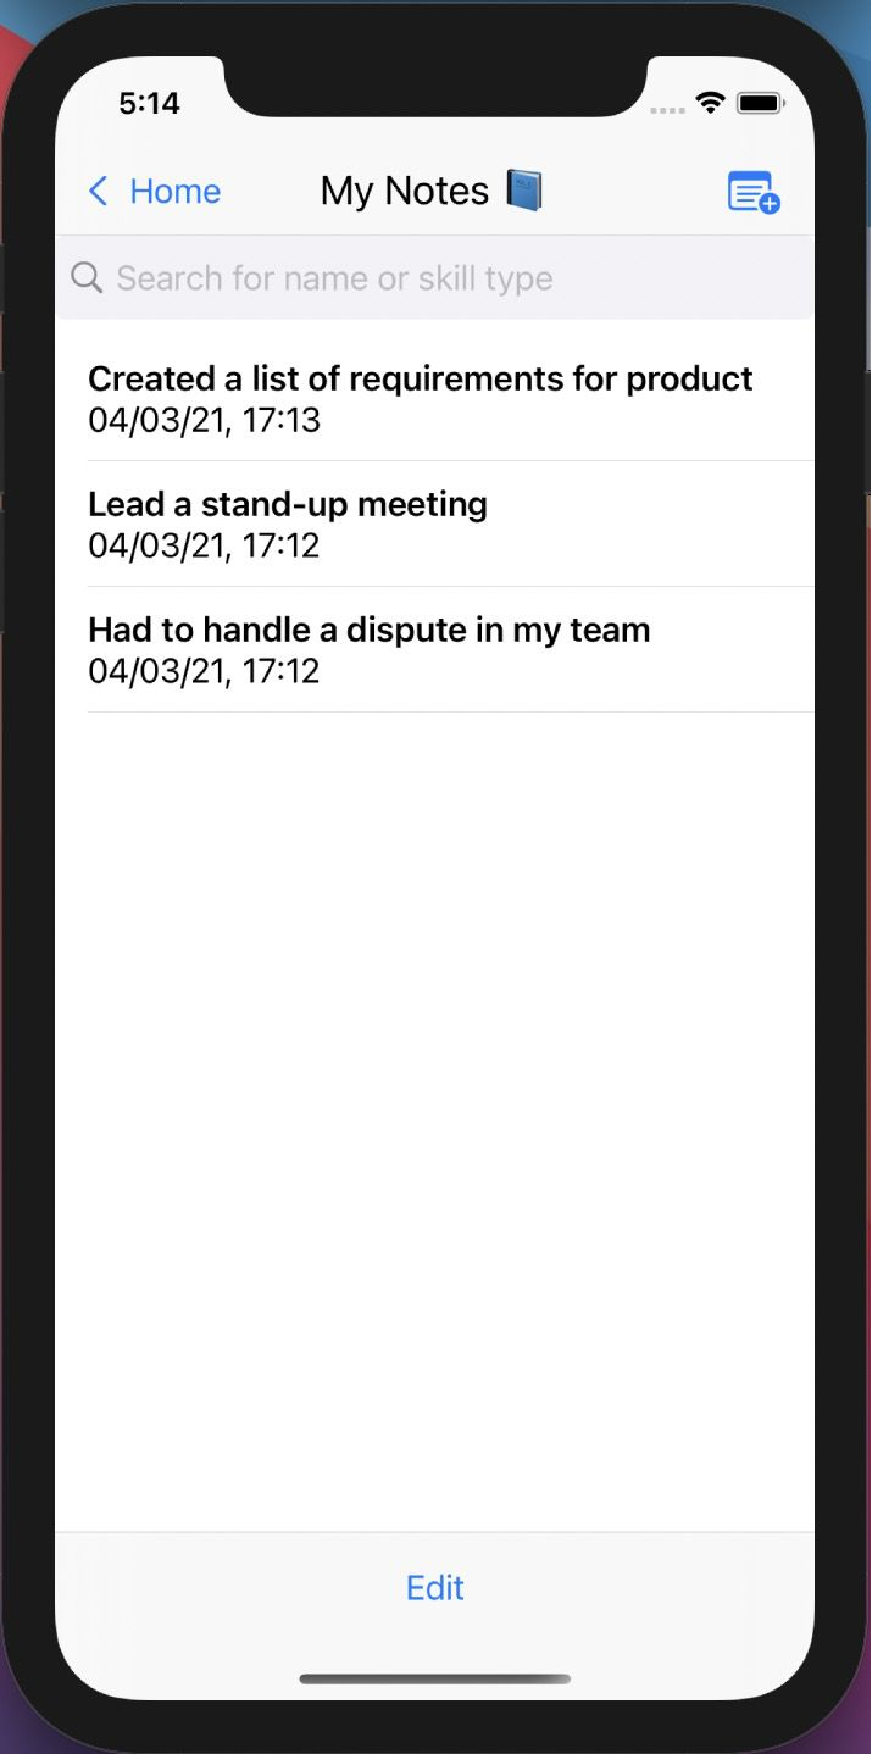
\includegraphics[scale=0.25]{images/appNotesScreen.pdf}
        \caption{Notes view}
        \label{fig:appNotesScreen}
    \end{subfigure}    
    \begin{subfigure}[b]{0.3\textwidth}
        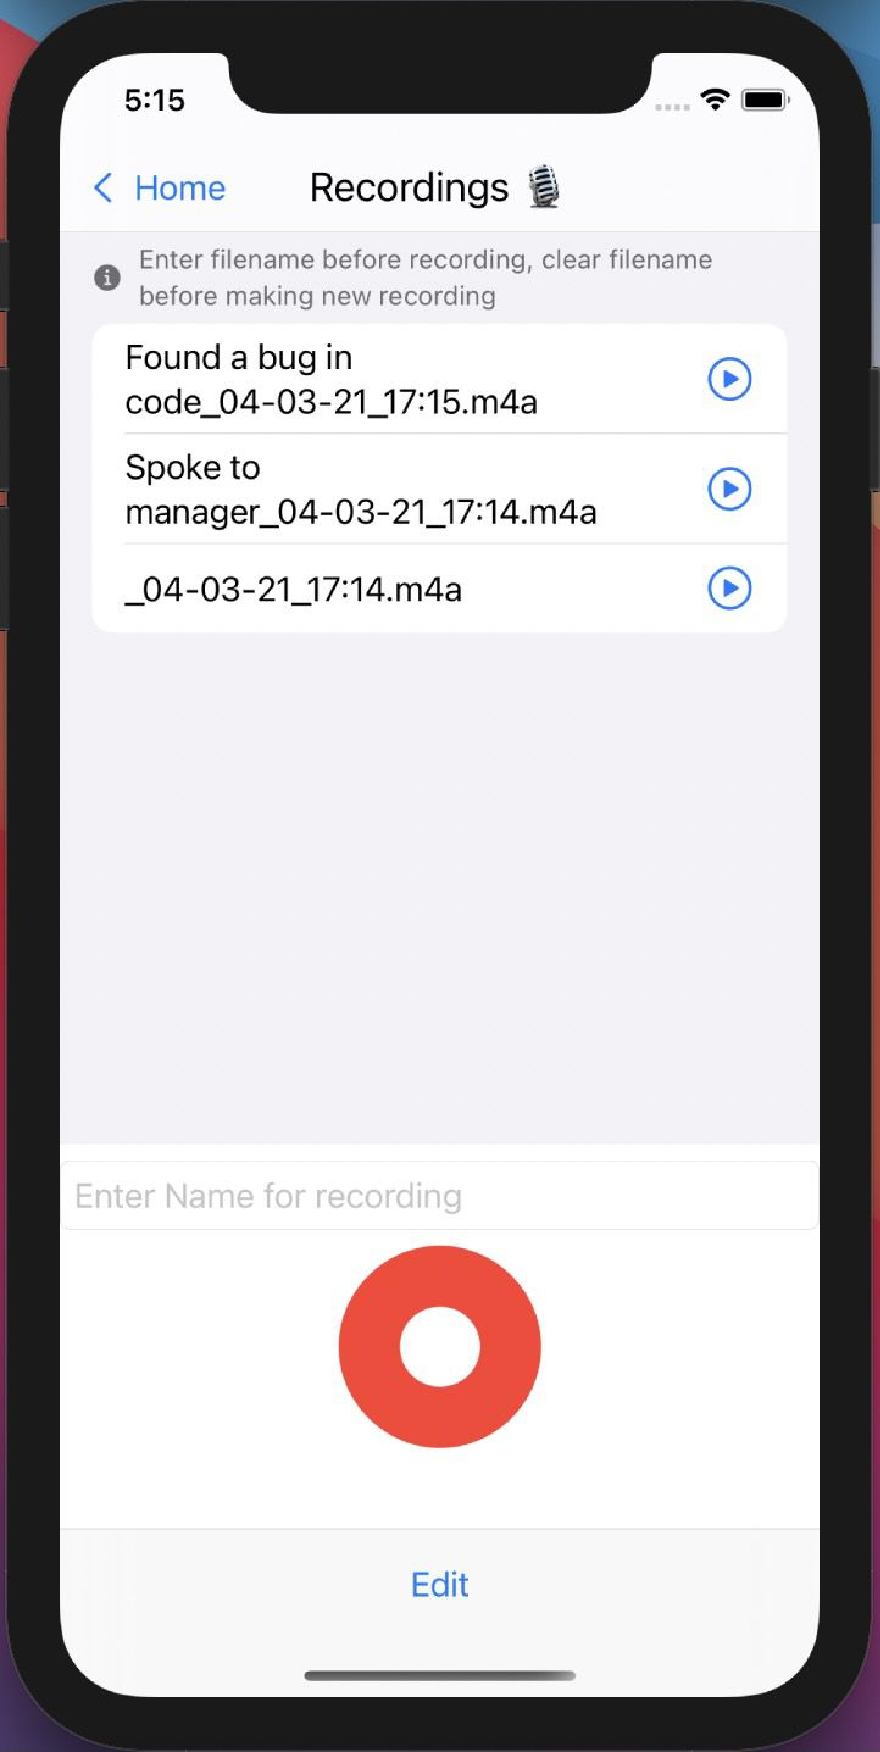
\includegraphics[scale=0.25]{images/appRecordingsScreen.pdf}
        \caption{Notes view}
        \label{fig:appRecordingsScreen}
    \end{subfigure} 
    \begin{subfigure}[b]{0.3\textwidth}
        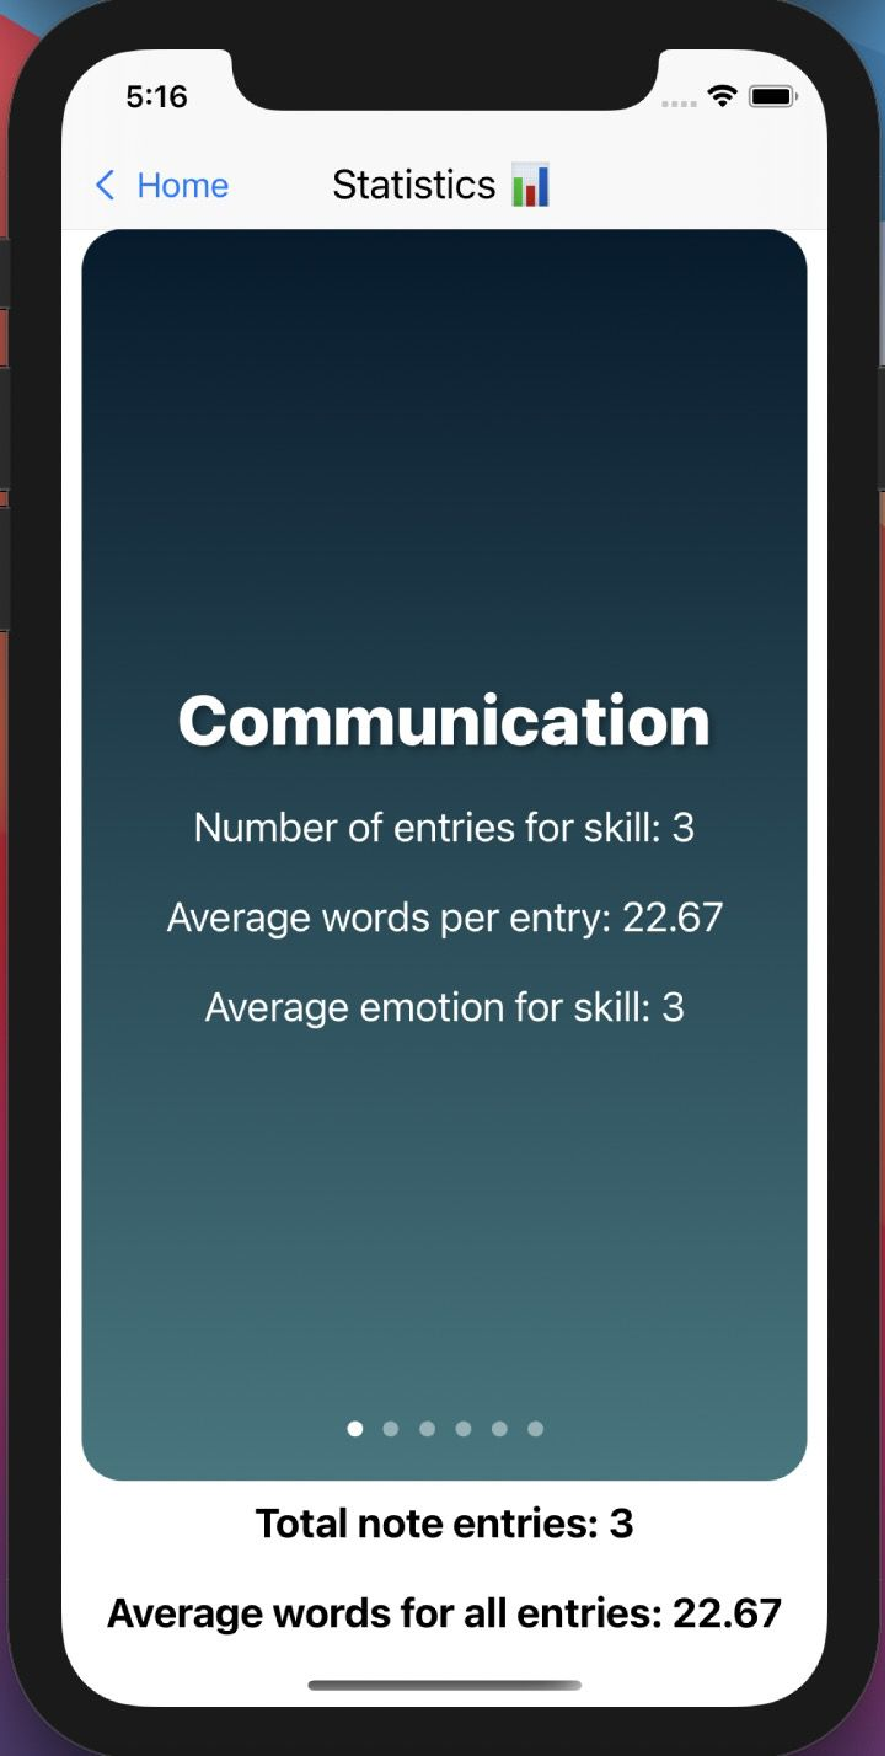
\includegraphics[scale=0.25]{images/appStatScreen.pdf}
        \caption{Statistics view}
        \label{fig:appStatScreen}
    \end{subfigure}  
    \begin{subfigure}[b]{0.3\textwidth}
        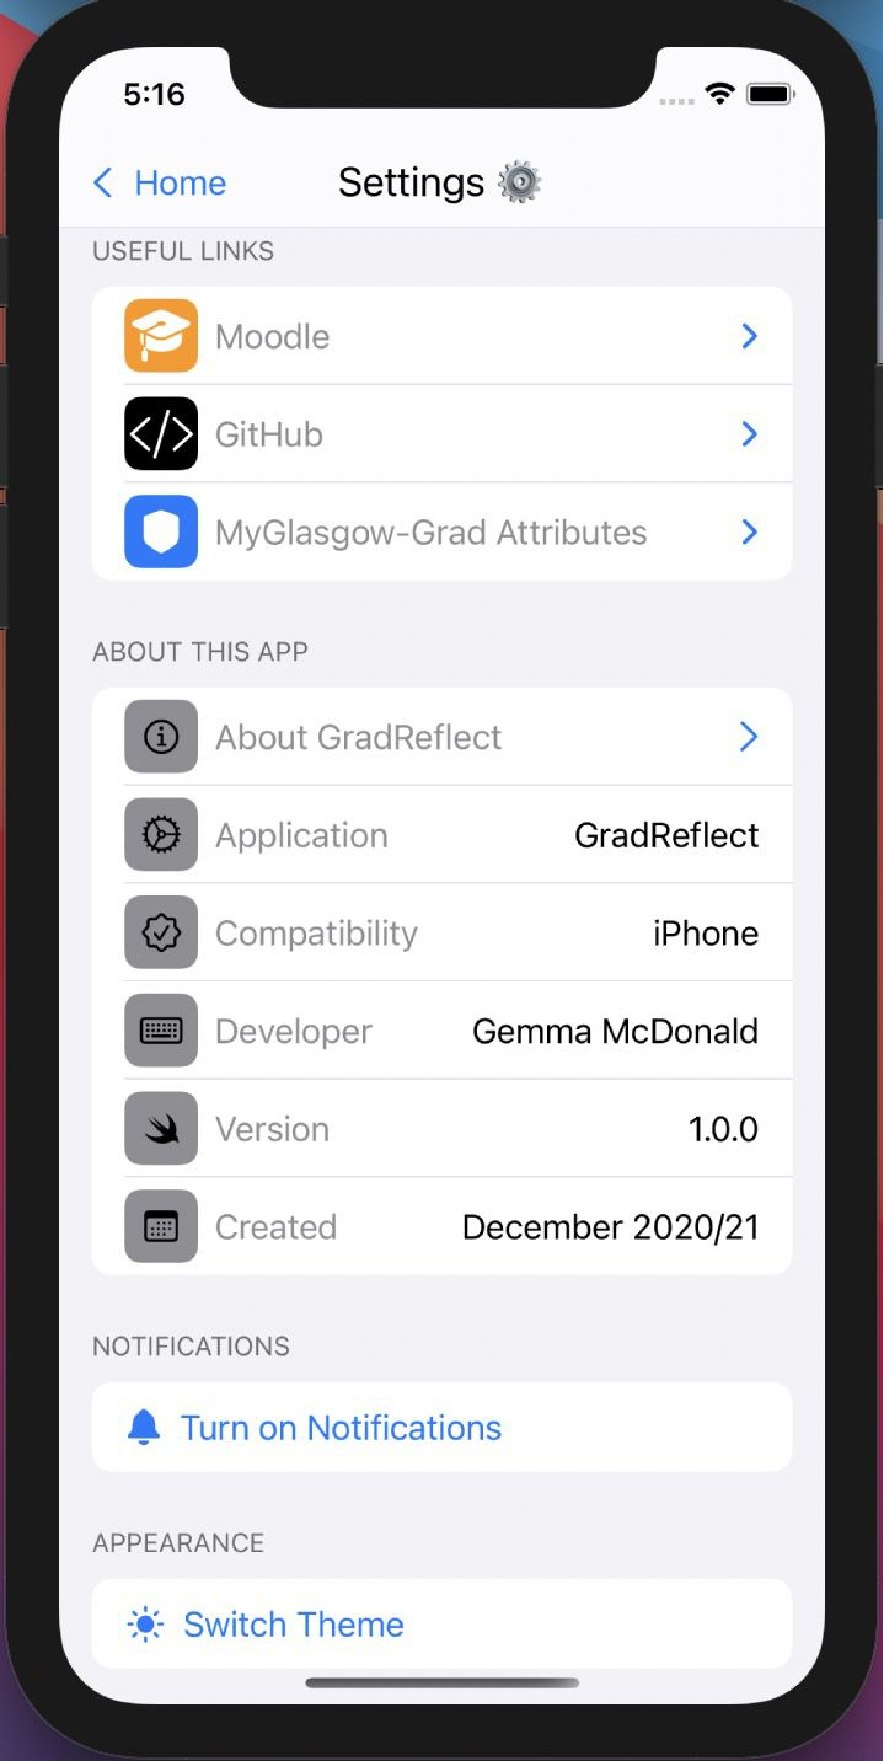
\includegraphics[scale=0.25]{images/appSettingsScreen.pdf}
        \caption{Settings view}
        \label{fig:appSettingsScreen}
    \end{subfigure}  
    \caption{Screenshots showing the main 5 views within the GradReflect application.}
    \label{fig:appMainViews}
\end{figure}

\subsection{Aesthetic features}

\textbf{Loading Screen:} A loading screen was created using the applications logo and colour scheme. This was to create a more professional and attractive looking application, whilst also performing the function of ensuring to the user that the application is loading, instead of a white screen which may lead the user to believe the application may have crashed.

\textbf{Emojis:} Emojis were implemented throughout the application. This was suggested by a potential user during early stages of development after they had viewed the progress of GradReflect. This was to create a more casual and friendly design to the application whilst also being informative of functionality. These emojis can be seen in the titles for views in figure \ref{fig:appMainViews}.

\textbf{App information in Settings:} Detail about the application such as name, compatibilty, developer, version and created date are provided in the settings section of the application. This is a common feature in iOS applications and gives a more professional design to the settings. These can be seen in figure \ref{fig:appSettingsScreen}

\textbf{Images on skill cards:} Each skill card contains a graphic that summarises the skill. These make the application more attractive and can add to a user's understanding of a skill. Many users pointed out that they enjoyed these images in the user evaluations conducted in chapter \ref{evaluation}. One of these images can be seen in figure \ref{fig:AdaptabilitySkillCard}.

\textbf{Toggle dark/light theme:} Users are able to toggle between dark and light theme within the application, this provides an element of customisability to the application for users, adding to usability and attractiveness. This dark mdoe can be seen in figure \ref{fig:DarkMode}, compared with the light mode that can be seen in figure \ref{fig:appMainViews}. 

\begin{figure}
    \centering
    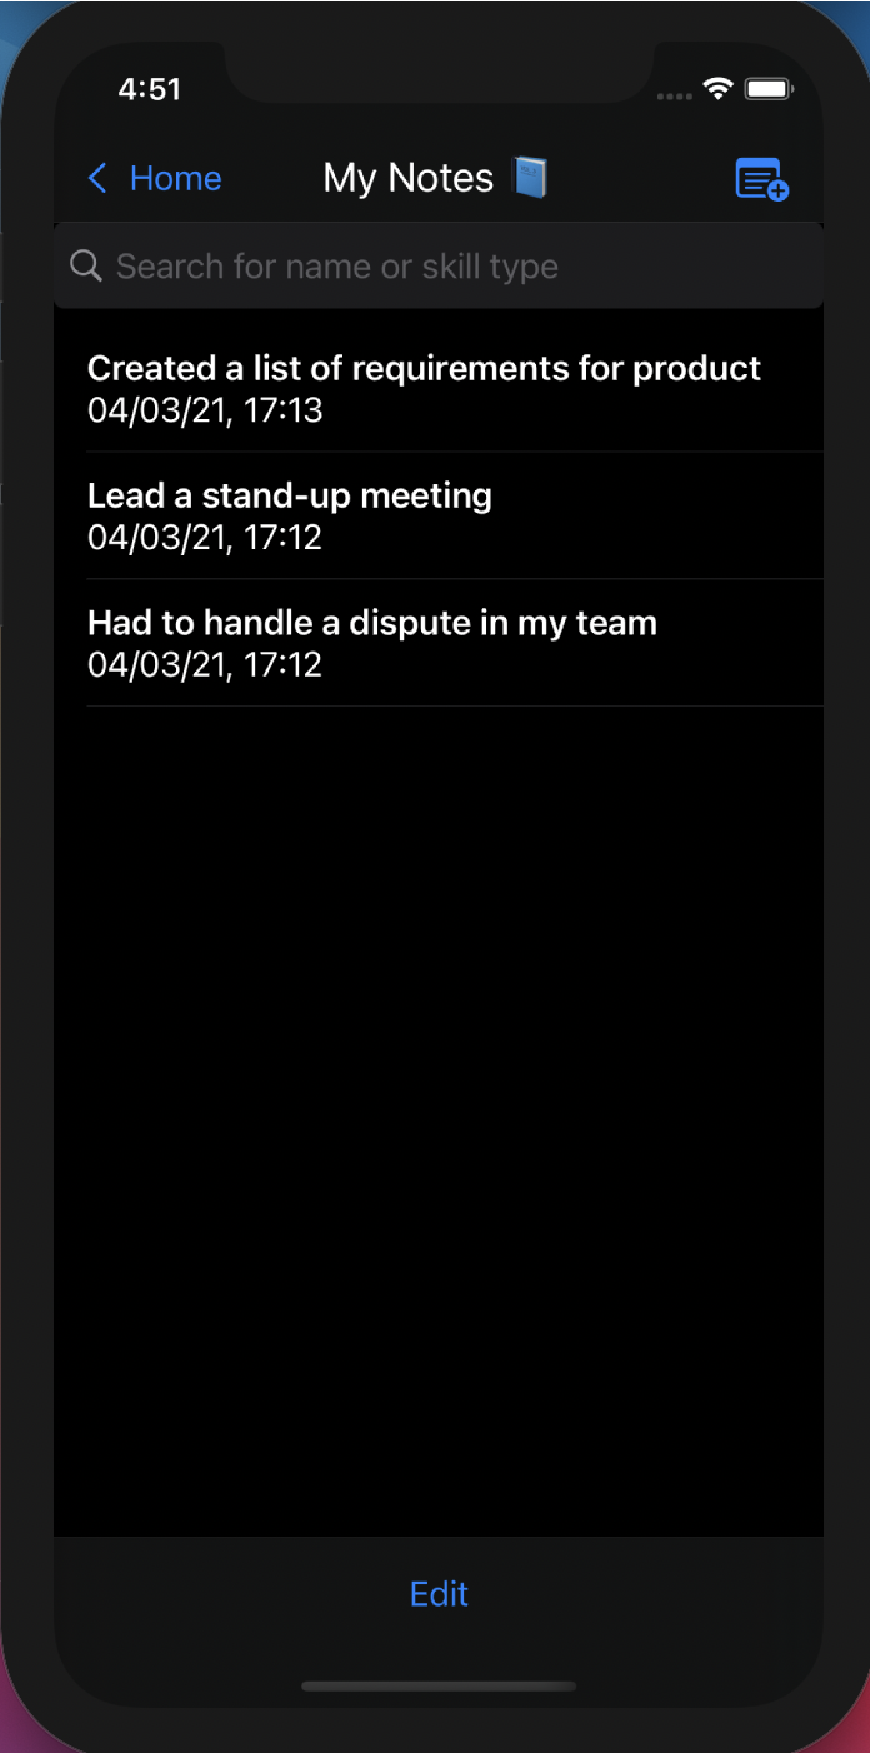
\includegraphics[scale=0.4]{images/DarkMode.pdf}    
    \caption{This screenshot shows the notification the notes view after the user has toggled to dark mode.}
    \label{fig:DarkMode} 
\end{figure}


\section{Features}

This section describes how the functional requirements for the system were implemented and lists some of the most 
important and relevant features. 
%     \item \textbf{MH} Allows for capturing of reflections in either text form OR audio form
%     \item \textbf{MH} Must have reminders
%     \item \textbf{MH} Be able to delete notes/audios
%     \item \textbf{MH} Be able to review/playback notes/audios that have been made
%     \item \textbf{SH} Be able to make BOTH text and audio form notes
%     \item \textbf{CH} Be able to view statistics based on the reflections recorded in the app
%     \item \textbf{CH} Have the ability to switch between dark and light theme on the app
%     \item \textbf{CH} Have a Settings page to view information about the app
%     \item \textbf{CH} Have an About Page that tells the user how to use the app correctly to make reflections
%     \item \textbf{CH} Have links in the Settings page that take you to useful pages related to the app and graduate attributes
%     \item \textbf{WH} Be able to upload reflections onto Moodle
%     \item Must be intuitive and easy to use. An application that is easier for new users is more likely to encourage users to continue
%     to use the application and have an interest in it.
%     \item Encourage the users to want to continue using the application for future uses, users should hopefully find the value in an
%     application similar to this. 

\subsection{Learn about graduate skills}

It is important for those who are wanting to reflect and develop their graduate attributes to learn and understand what these skills actually are before reflection. Users are able to swipe through the skill cards on the home section of the application to view a helpful graphic and description of the skill and where someone could potentially use it. An example of one of these skill cards can be seen in figure \ref{fig:AdaptabilitySkillCard}. This was done to help users feel more comfortable in their reflections and not feel daunted by having to choose a skill to reflect on as they already know and understand what all of these skills are. These skill descriptions were placed on the home section of the application so that new users to the application can instantly scroll to familiarise themselves with the skills they can expect to develop through the use of the application. Experienced users do not have to scroll anywhere and can immediately choose where in the application they want to navigate, however still have the option of a convenient reminder of these skills should they require it. 

\begin{figure}
    \centering
    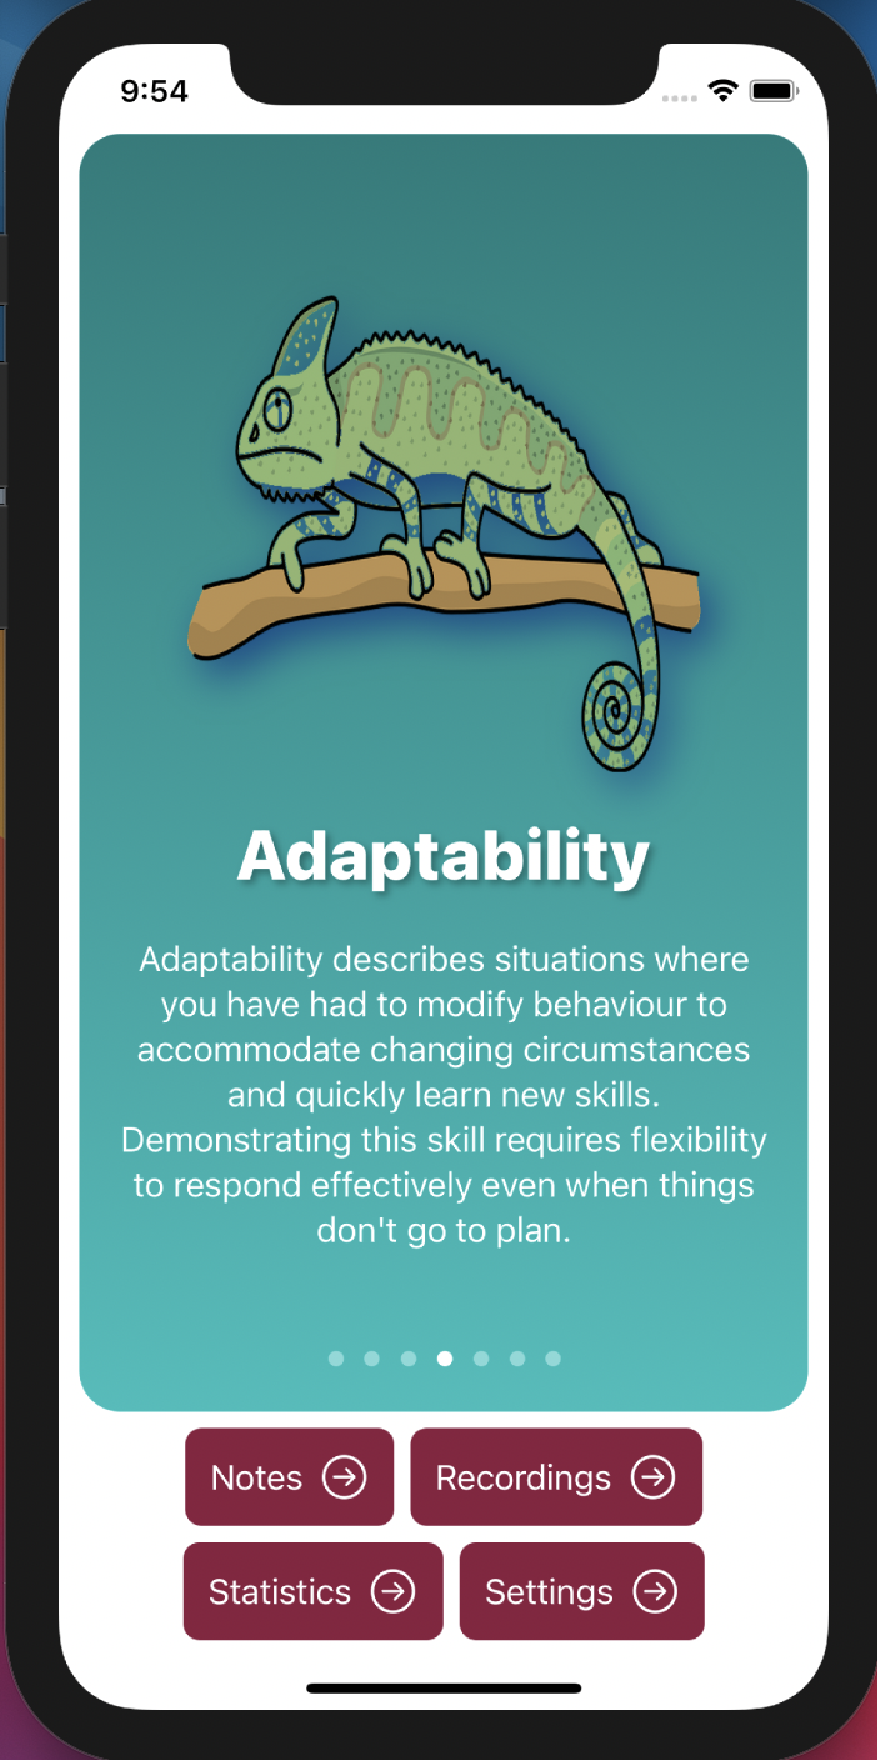
\includegraphics[scale=0.4]{images/AdaptabilitySkillCard.pdf}    
    \caption{This screenshot shows the Adaptability skill card, one of the 6 skill descriptions available on the Home view of the GradReflect application.}
    \label{fig:AdaptabilitySkillCard} 
\end{figure}

\subsection{Creating and deleting a note}

The ability to capture a reflection in written form was a key functional requirement for this project. One thing that makes this project stand out from similar existing note or reflective applications is the utilisation of Cognitive Behavioural Therapy (CBT) techniques that are used to provide the scaffolding needed to support users in this reflection. This was implemented through the note creation form, users are able to create and save a new note and carry out their reflection using the question prompts provided for them. This form can be seen in figure \ref{fig:CreatingNote}. This aims to give clear instructions to focus the user on reaching all stages of reflection and therefore increasing their likelihood of development of these skills as it increases their situational awareness and reflective abilities. 

The user was also supported in their reflection through the use of help buttons. The user is able to click on the '?' button next to any of the questions in the note entry form and an alert will appear that provides further detail on how they are expected to answer the question. An example of this alert can be seen in figure \ref{fig:HelperButtonAlert}. Throughout each of the help button alerts, the example of a communication skill reflection is used where someone has had to settle a dispute in their team. Examples are given in each of the alerts using this situation as an example of the sort of reflections the user could make.

Users can select one of the 6 skills available to reflect on from a picker, ensuring conformity in the skills so that there are no issues when users later are
able to search for a skill to filter their notes. Users are also able to select their emotional response to a situation using a slider, simplifying this
reflection for them. 

Users are able to save a note after reflecting, however, this cannot be done without a title given. This was intended to give the user freedom in how much they did or did not want to write. They are also able to cancel a note at any given time by either click the cancel button or swiping from the top down to dismiss the form. 

Users can later delete a note by either selecting the edit button, or through swiping a note in the list to the left. The edit mode for notes can be seen in figure \ref{fig:DeleteNote}. This is a native gesture in iOS used frequently in other applications. Users are unable to update or edit a note after its creation however, as this would replicate the CBT practices or writing in a journal, where relfections cannot be edited. 

\begin{figure}
    \centering
    \begin{subfigure}[b]{0.3\textwidth}
        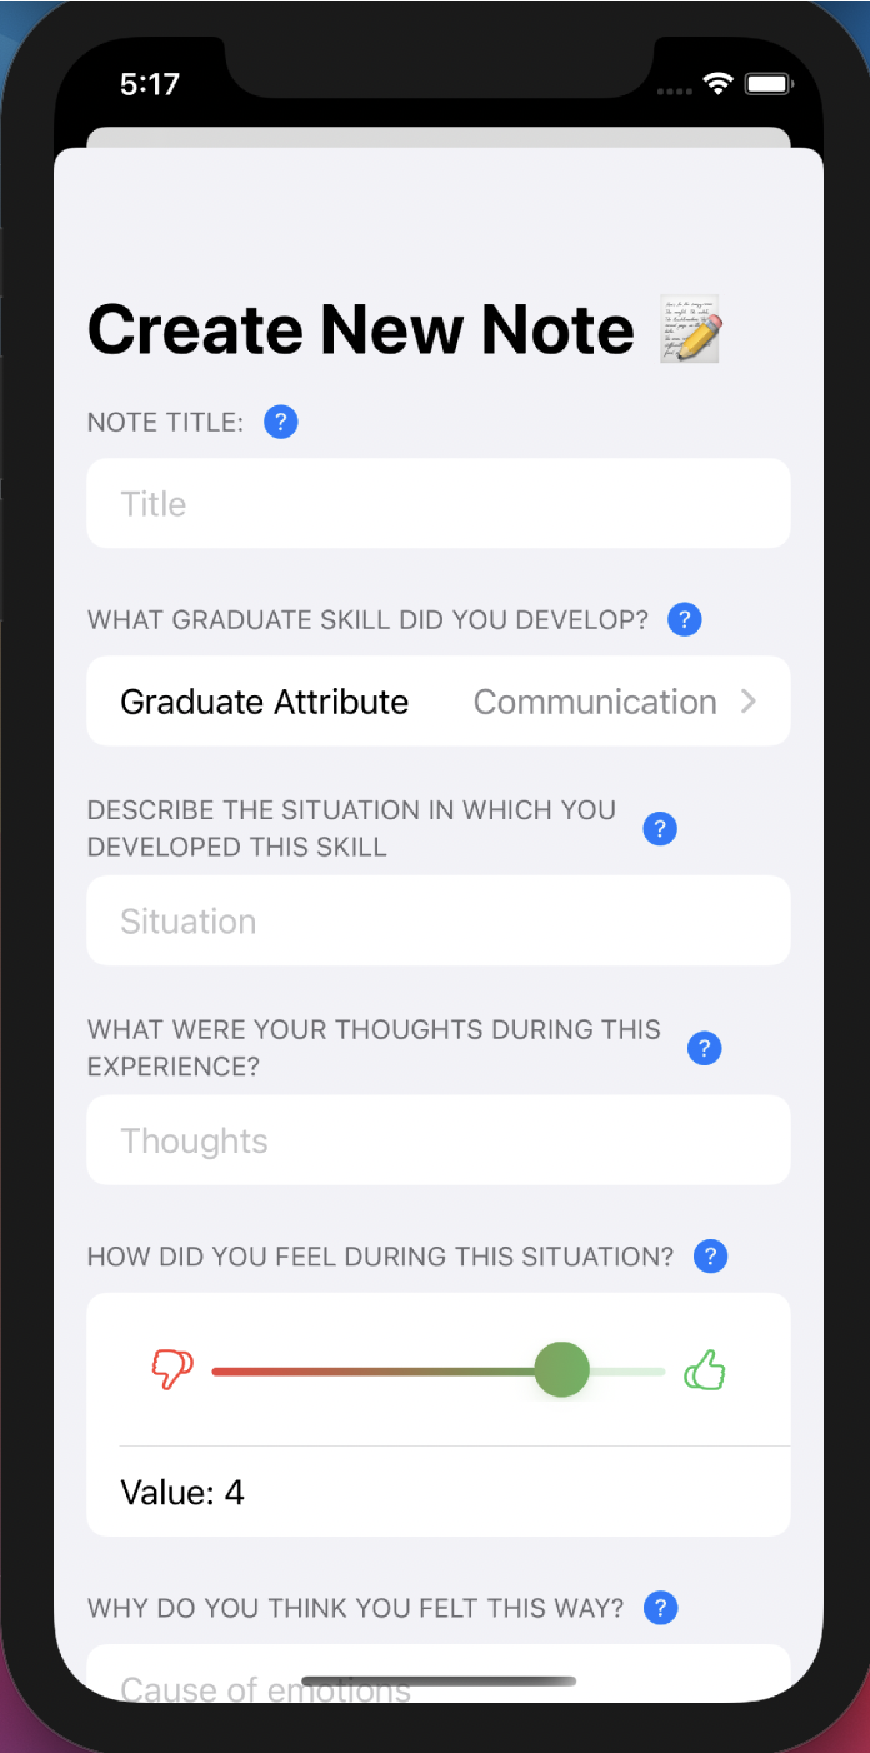
\includegraphics[scale=0.25]{images/CreatingNote.pdf}
        \caption{Form to create a note.}
        \label{fig:CreatingNote}
    \end{subfigure}
    \begin{subfigure}[b]{0.3\textwidth}
        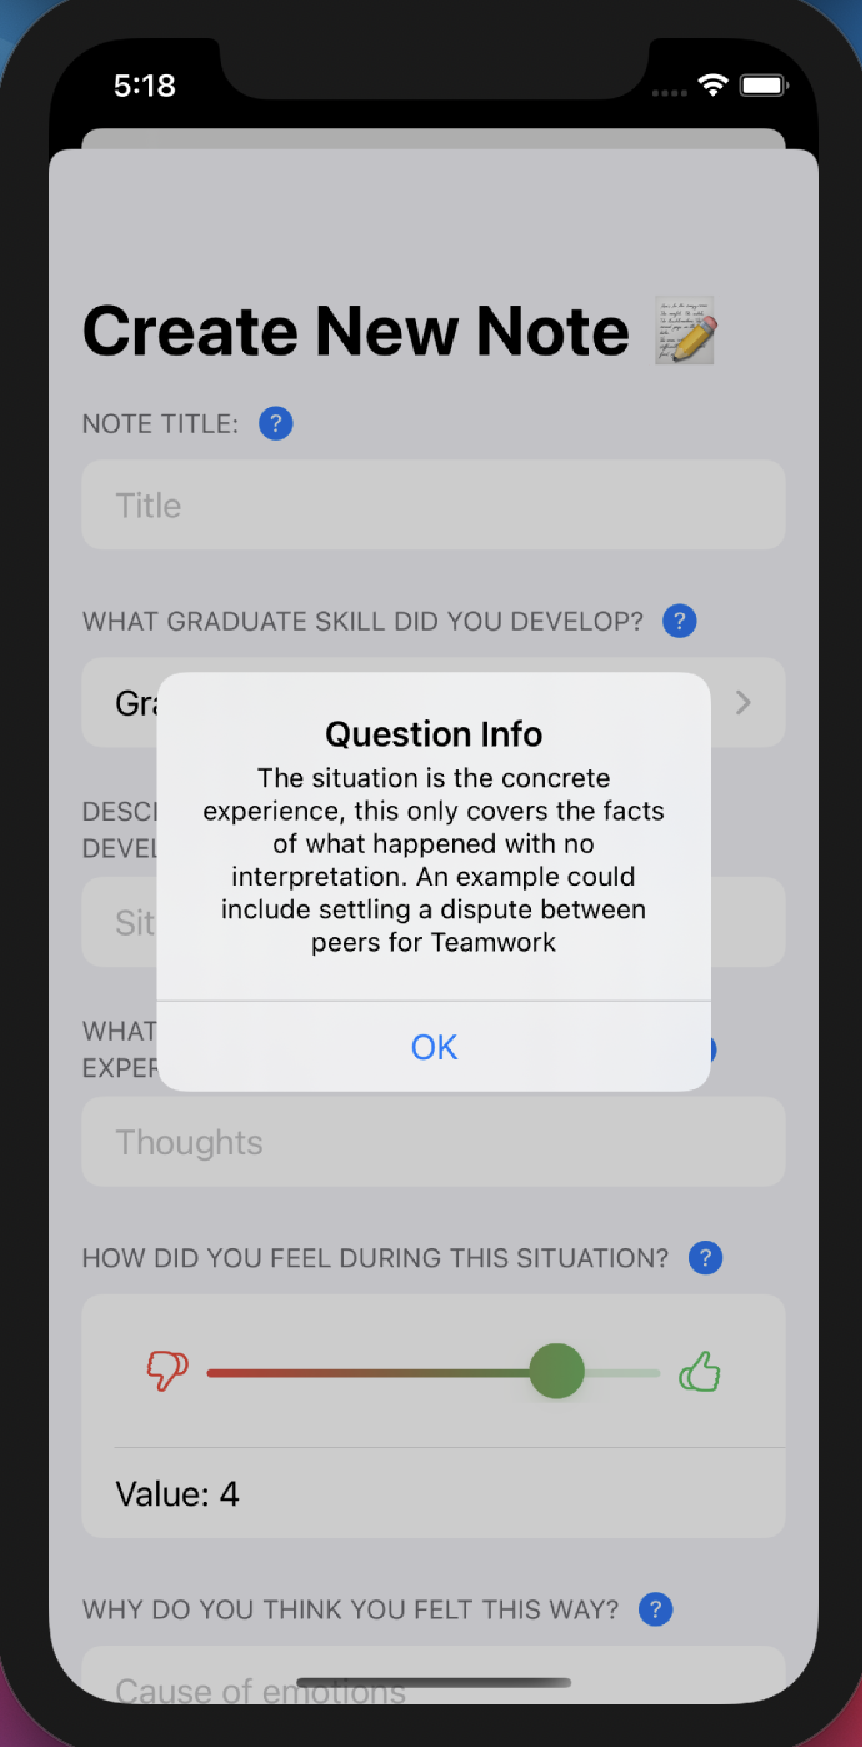
\includegraphics[scale=0.25]{images/HelperButtonAlert.pdf}
        \caption{Alert given from the situation prompt by help button.}
        \label{fig:HelperButtonAlert}
    \end{subfigure}   
    \begin{subfigure}[b]{0.3\textwidth}
        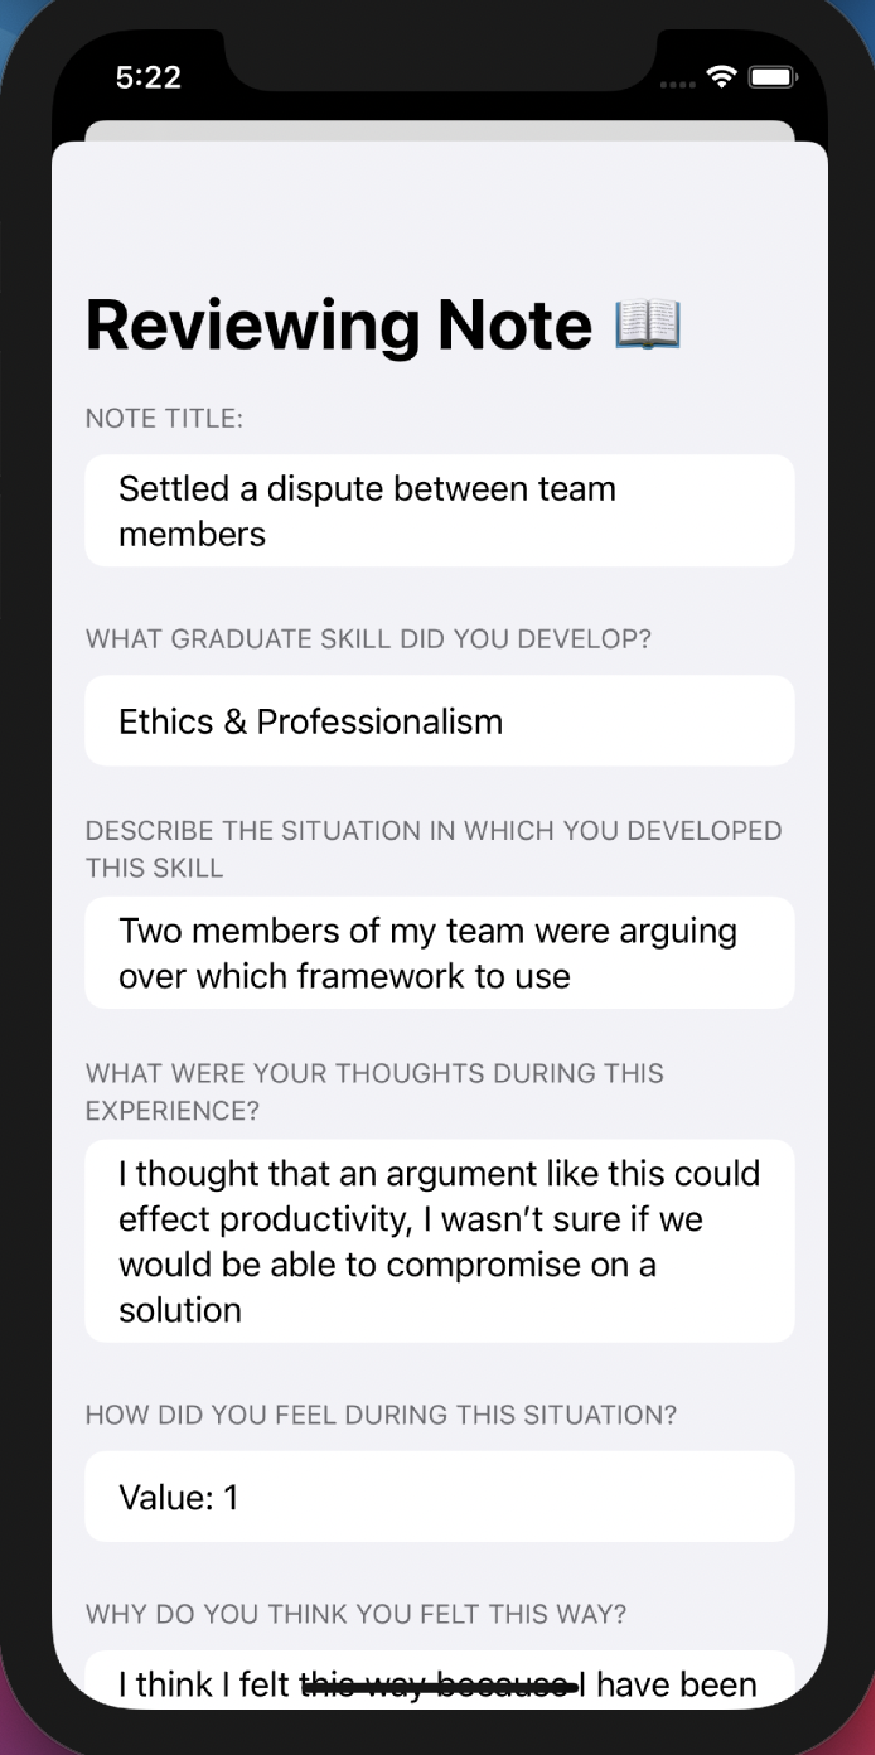
\includegraphics[scale=0.25]{images/ReviewingNote.pdf}
        \caption{Reviewing a note}
        \label{fig:ReviewingNote}
    \end{subfigure}   
    \caption{Screenshots showing the views when creating a note and reviewing it.}
    \label{fig:NoteCreationReview}
\end{figure}

\subsection{Reviewing a note}

Users are able to click on a previous note they have made, allowing them to reflect on previous events and their reflections. This could enable them to see how they have improved or handled previous similar scenarios. This can be seen in figure \ref{fig:ReviewingNote}.

\subsection{Search and filter}

Users are able to type in the name of a note to filter the list of notes presented, shown in figure \ref{fig:SearchFilter}. They are also able to type in a specific skill to filter the list by that skill. This is a useful feature as it is intended that users would continue to use this application frequently to reflect, and therefore having the ability to filter notes would make it easier for them to find previous notes they have made for a skill. 

\begin{figure}
    \centering
    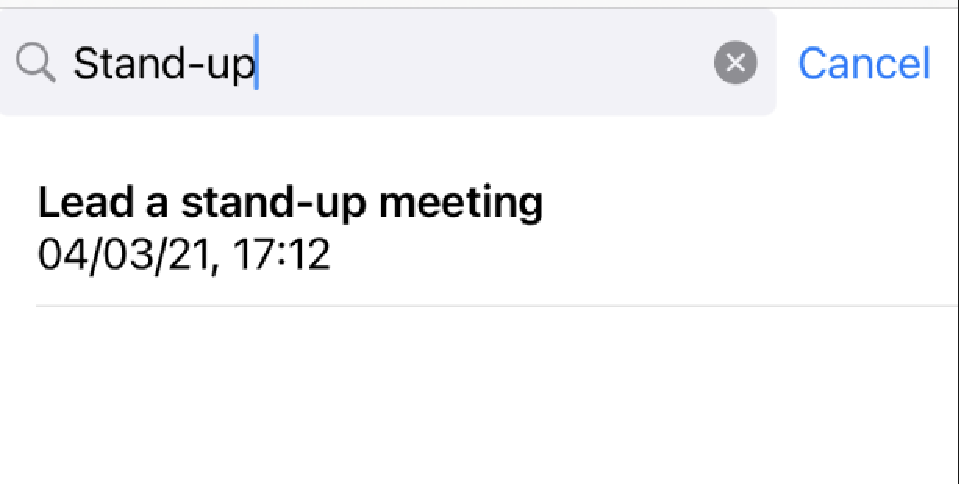
\includegraphics[scale=0.4]{images/SearchFilter.pdf}    
    \caption{This screenshot shows the list filtered after searching for a term in the name of one of the notes.}
    \label{fig:SearchFilter} 
\end{figure}

\subsection{Record an audio}

Users are also able to record an audio of themselves discussing a situation or skill. This provided a more convenient option, with the freedom to discuss anything the user wishes to. An AVAudioRecorder provided the recording capabilities within the application, using the user-built-in microphone and speaker. SwiftUI provides a strict format for creation audio capabilities within an application, this is intended to reduce programming overhead. An AVAudioSession is used to configure the audio session of the application. Each time a recording started a new audio session is created and set to the category playAndRecord, meaning that a user is able to create and recording and play it back. It ensures that the application will conform to typical iOS behaviours, such as muting a record upon locking the device, or silencing other background audio when a recording is played. 
Users are able to start a recording until they click stop, the recording button can be seen in figure \ref{fig:appRecordingsScreen}. AVAudioRecorder will be given the provided name from the user if they had entered it in the naming field prior to clicking record, or will set the name of the recording to the date and time of creation if the user does not provide a name. 

\subsection{Playback and delete recording}

Users are able to playback a recording, allowing them to convert this recording into a fully written note, this playback button can be seen in figure \ref{fig:appRecordingsScreen}. They can then delete any notes in the same way as a written note via either the edit button or swiping to the left. Edit mode for this can be seen in figure \ref{fig:DeleteAudio}.

\begin{figure}
    \centering
    \begin{subfigure}[b]{0.3\textwidth}
        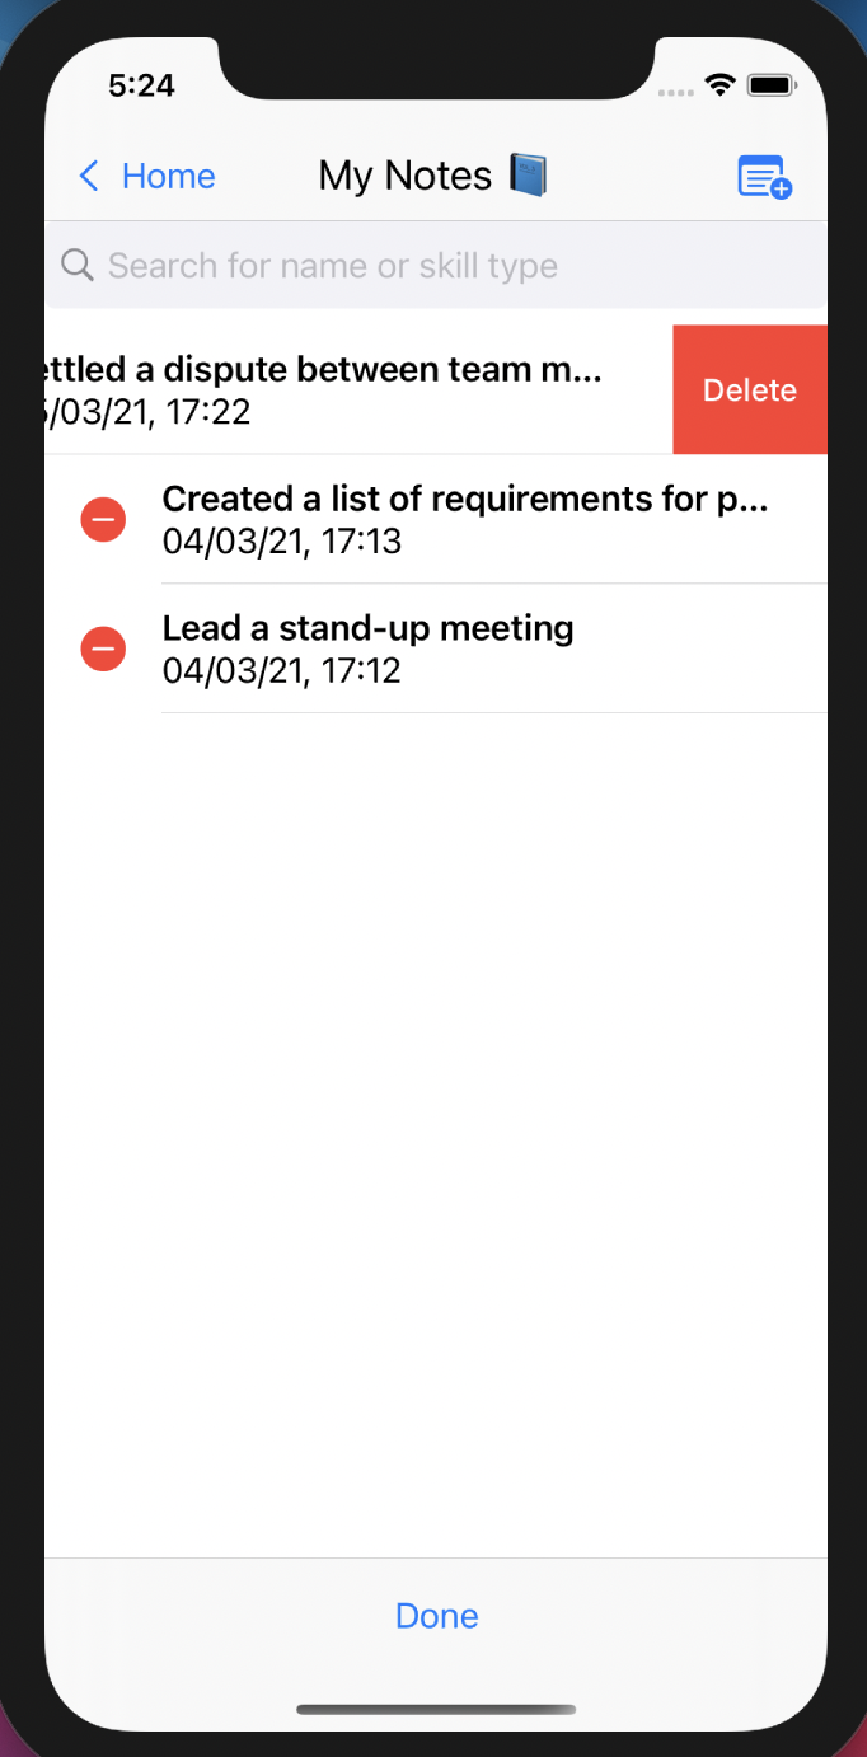
\includegraphics[scale=0.25]{images/DeleteNote.pdf}
        \caption{Delete note.}
        \label{fig:DeleteNote}
    \end{subfigure}
    \begin{subfigure}[b]{0.3\textwidth}
        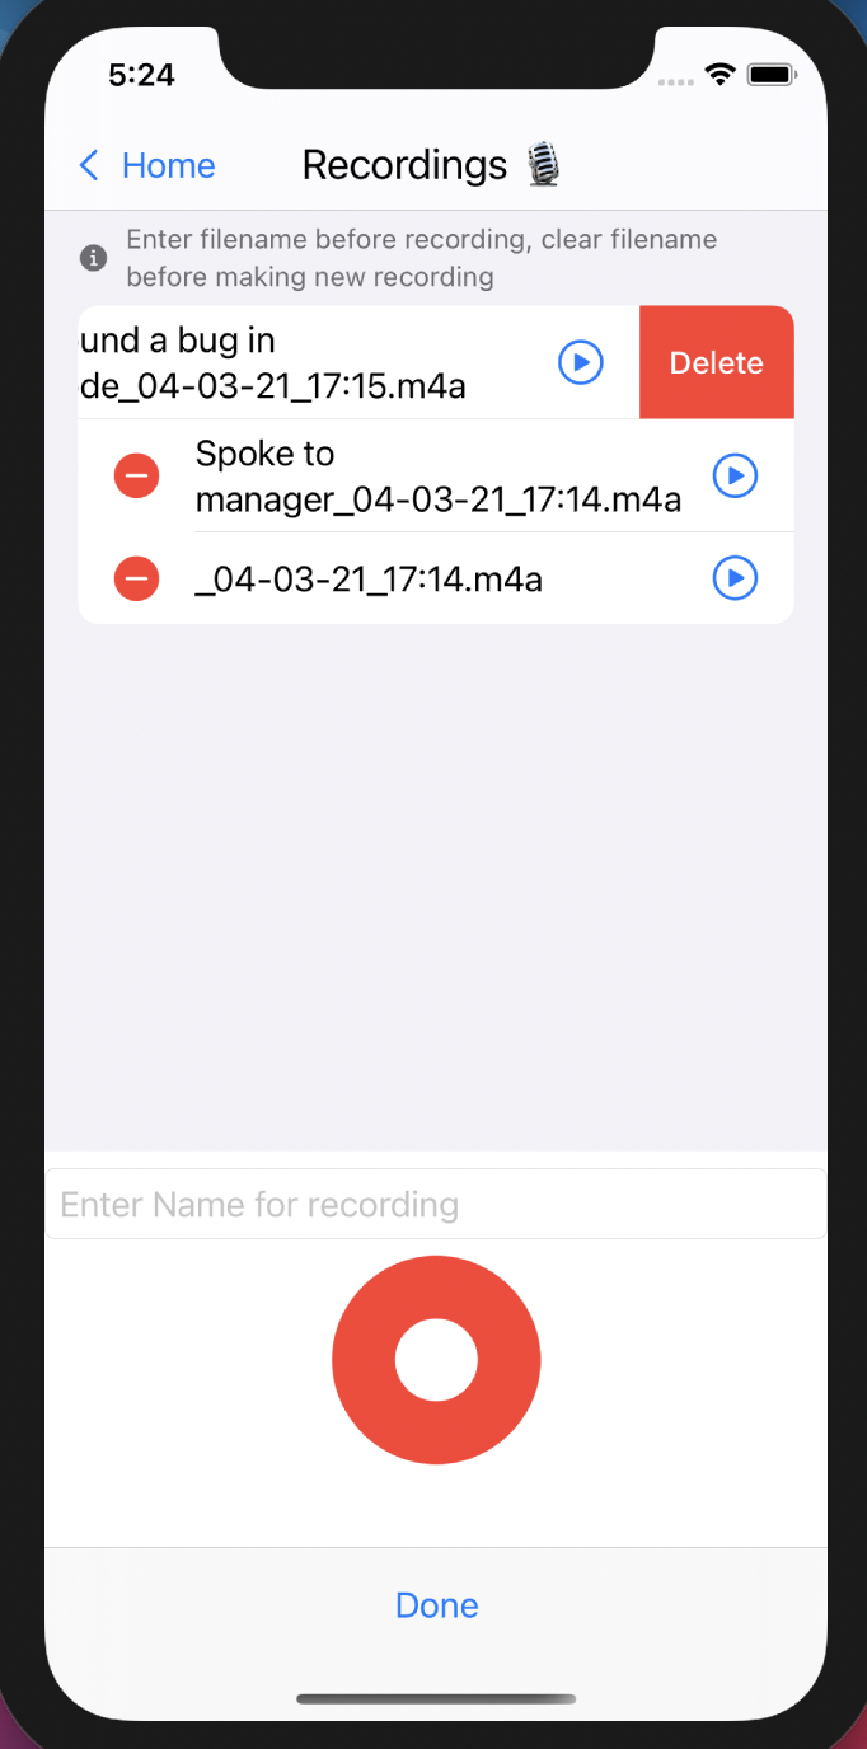
\includegraphics[scale=0.25]{images/DeleteAudio.pdf}
        \caption{Delete audio.}
        \label{fig:DeleteAudio}
    \end{subfigure}   
    \caption{Screenshots showing the edit mode allowing deletion.}
    \label{fig:Deletion}
\end{figure}

\subsection{Review statistics}

Users are able to view the statistics of their notes, seen in figure \ref{fig:appStatScreen}. Each skill is presented with the same colour scheme used in the skill descriptions to ensure a cohesive look to the application. Each skill card contains the number of notes they have made on the skill, the average words per entry, and their average emotional response for the skill. Users are also able to view their total number of notes and their average word per note over every note. This was to allow the user to make comparisons between each skill and how extensively they had reflected in their notes and how they generally view experiences that engage this skill. The average emotion over all skills was not given as a metric as it was decided that this woud not be useful to users as it is more useful to review how they feel about a specific skill rather than over all experiences. 

\subsection{Visit useful links}

The Settings view also provides users with links that could potentially assist them in their reflections. One of the links given takes the user to the University of Glasgow website on graduate attributes, linking this project to the university and how it expects them to develop these skills throughout htier education. A link was also given to the University of Glasgow's Moodle page. This was as exporting reflections to Moodle had been considered during the requirements gathering stage but had been decided was not useful as users may not have the desire to upload these reflections onto Moodle due to their personal nature of the users experiences and emotions. SwiftUI and iOS development also did not provide a Moodle API to allow users to do this. Instead, a link is now given to users as an option so that they are able to take their reflections to Moodle themselves should they wish to. These links can be seen in figure \ref{fig:appSettingsScreen}.

\subsection{Notifications}

Users are able to turn on notifications through the Settings view. This was implemented using a UNUserNotificationCenter object, which manages all notification related activities for any application. Similarly to enabling recordings, SwiftUI provides a standard structure that notifications are allowed to be set up and enabled. The UNUserNotificationCenter manages the request of permission for GradReflect to send notifications to the user and scheduling when these notifications can occur. In the implemented application, the user is able to click to turn on notifications, this will set a notification to fire 10 seconds after pressing. This is to give the user enough time to close the applciation and wait for the incoming notification. The scheduling of 10 seconds is due to the application not going into real-world deployment, and is so that the ability for notifications can be tested during demonstrations and evaluations. For future deployment, the notifications would fire weekly, as this has been stated as the recommended timescale to regularly reflect \citep{bruno_reflective_2018}. The notification can be seen in figure \ref{fig:Notification}.

\begin{figure}
    \centering
    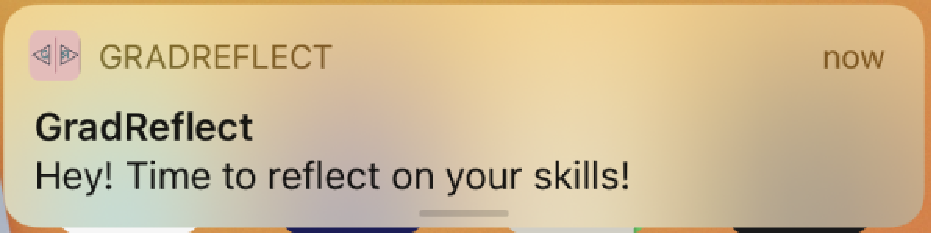
\includegraphics[scale=0.4]{images/Notification.pdf}    
    \caption{This screenshot shows the notification that fires after the user turns on notifications.}
    \label{fig:Notification} 
\end{figure}

\subsection{About GradReflect page}

Users were also able to navigate to an about GradReflect view through the Settings view. This was a simple description in detail of each aspect of the application and how the application was intended to be used. This section also describes to the user about the use of CBT within the application and how this is intended to assist them. The goal of this page is to provide users with further clarifications of how they can use the application to develop their skills and provide greater detailed instructions and support necessary for them to be able to reflect effectively. This page can be seen in figure \ref{fig:AboutApp}.

\begin{figure}
    \centering
    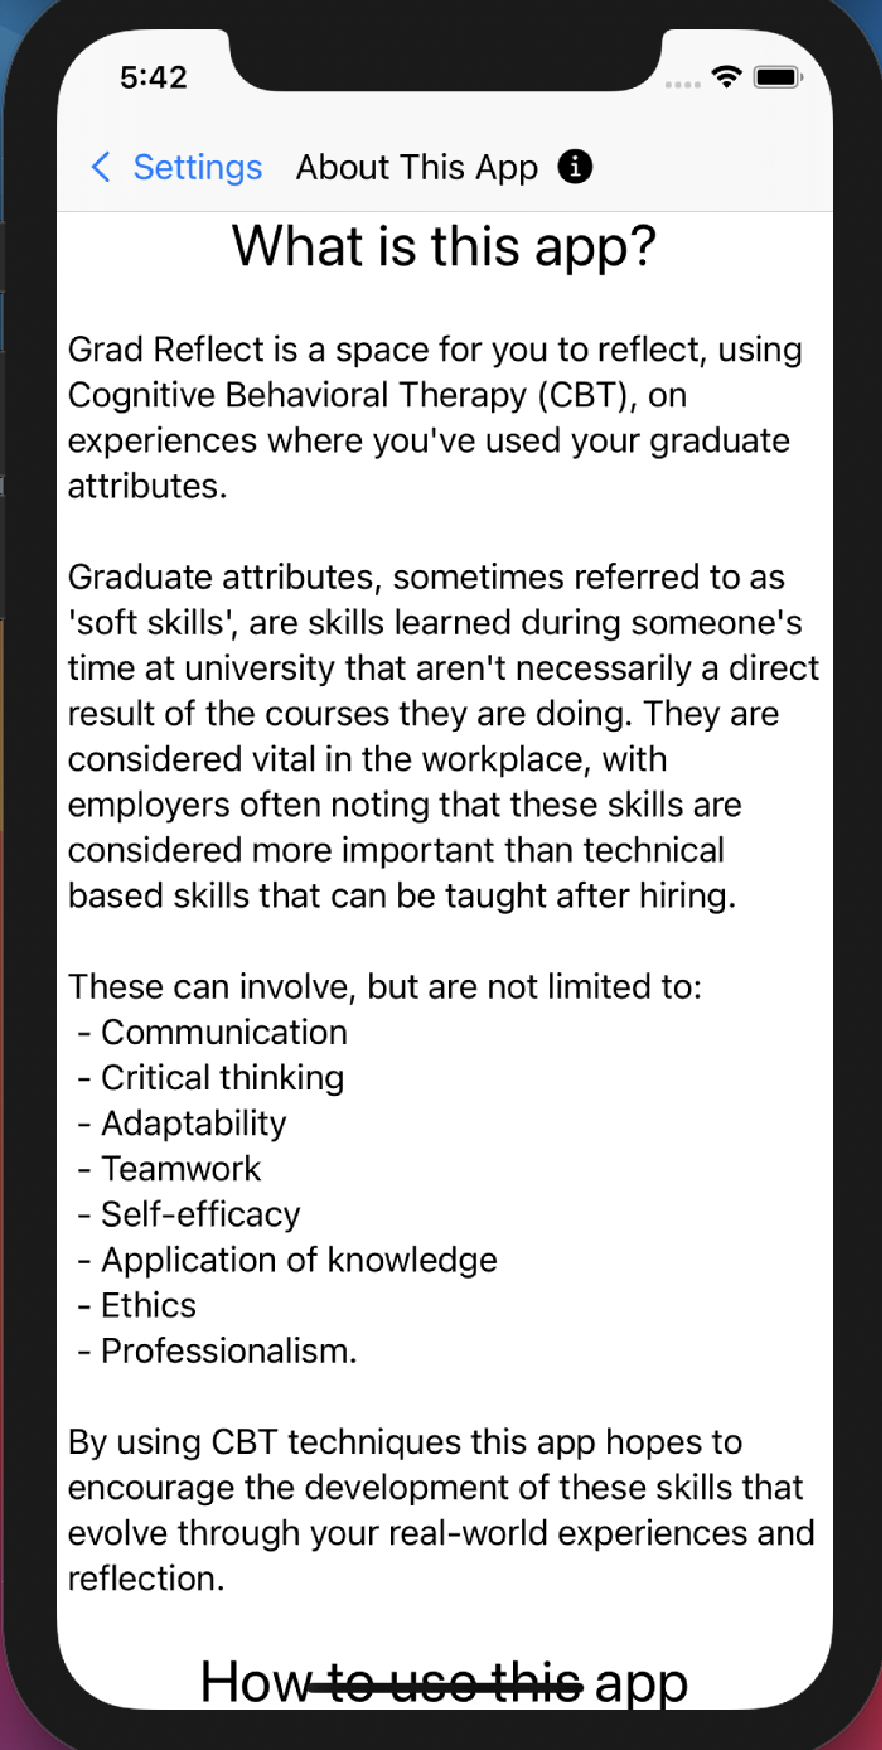
\includegraphics[scale=0.4]{images/AboutApp.pdf}    
    \caption{This screenshot shows the About GradReflect page.}
    \label{fig:AboutApp} 
\end{figure}

\section{Maintainability}
An important goal for the project was to allow future developers to maintain the project and to add new features, eventually taking this application into 
deployment through the app store and potentially making a cross-platform version to allow users with any mobile operating system. Steps were taken to ensure that 
the code and documentation were of high enough quality to allow this, these steps are listed below.

\subsection{Documentation}

\textbf{Code Commentary} Code commentary was used through the implementation process to ensure that it was always clear what the purpose of the code was. Upon
copletion of the project this commentary was further developed into a narrative throughout the code to show the links between views, functionality, and where
data is being passed. This will allow any future developers to quickly understand how the application was made, fix buds, and add new features.

\textbf{GitHub Wiki} Throughout the course of the project, the GitHub wiki was kept up to date with weekly progress, meetings and research. The wiki also 
contained the goals and requirements for the project. This meant that anyone reading the wiki is able to easily understand the objectives of the application
and the research that went into the design of the questions and the intentions behind reflection and developing user graduate attributes. This understanding
would help any future developers carry through these intentions into their own further development of the application, maintain the key goals at the core
of development. 

\textbf{Developer readme} A readme for developers is also included in the project. This explains how to set up the project for continued development and how
to run the application both on XCode Simulator and on their own iPhone. This is intended to make it easier for any future developers to create new features
to the application. 


% \subsection{Tables}

% If you need to include tables, like Table \ref{tab:operators}, use a tool like https://www.tablesgenerator.com/ to generate the table as it is
% extremely tedious otherwise. 

% \begin{table}[]
%     \caption{The standard table of operators in Python, along with their functional equivalents from the \texttt{operator} package. Note that table
%     captions go above the table, not below. Do not add additional rules/lines to tables. }\label{tab:operators}
%     %\tt 
%     \rowcolors{2}{}{gray!3}
%     \begin{tabular}{@{}lll@{}}
%     %\toprule
%     \textbf{Operation}    & \textbf{Syntax}                & \textbf{Function}                            \\ %\midrule % optional rule for header
%     Addition              & \texttt{a + b}                          & \texttt{add(a, b)}                                    \\
%     Concatenation         & \texttt{seq1 + seq2}                    & \texttt{concat(seq1, seq2)}                           \\
%     Containment Test      & \texttt{obj in seq}                     & \texttt{contains(seq, obj)}                           \\
%     Division              & \texttt{a / b}                          & \texttt{div(a, b) }  \\
%     Division              & \texttt{a / b}                          & \texttt{truediv(a, b) } \\
%     Division              & \texttt{a // b}                         & \texttt{floordiv(a, b)}                               \\
%     Bitwise And           & \texttt{a \& b}                         & \texttt{and\_(a, b)}                                  \\
%     Bitwise Exclusive Or  & \texttt{a \textasciicircum b}           & \texttt{xor(a, b)}                                    \\
%     Bitwise Inversion     & \texttt{$\sim$a}                        & \texttt{invert(a)}                                    \\
%     Bitwise Or            & \texttt{a | b}                          & \texttt{or\_(a, b)}                                   \\
%     Exponentiation        & \texttt{a ** b}                         & \texttt{pow(a, b)}                                    \\
%     Identity              & \texttt{a is b}                         & \texttt{is\_(a, b)}                                   \\
%     Identity              & \texttt{a is not b}                     & \texttt{is\_not(a, b)}                                \\
%     Indexed Assignment    & \texttt{obj{[}k{]} = v}                 & \texttt{setitem(obj, k, v)}                           \\
%     Indexed Deletion      & \texttt{del obj{[}k{]}}                 & \texttt{delitem(obj, k)}                              \\
%     Indexing              & \texttt{obj{[}k{]}}                     & \texttt{getitem(obj, k)}                              \\
%     Left Shift            & \texttt{a \textless{}\textless b}       & \texttt{lshift(a, b)}                                 \\
%     Modulo                & \texttt{a \% b}                         & \texttt{mod(a, b)}                                    \\
%     Multiplication        & \texttt{a * b}                          & \texttt{mul(a, b)}                                    \\
%     Negation (Arithmetic) & \texttt{- a}                            & \texttt{neg(a)}                                       \\
%     Negation (Logical)    & \texttt{not a}                          & \texttt{not\_(a)}                                     \\
%     Positive              & \texttt{+ a}                            & \texttt{pos(a)}                                       \\
%     Right Shift           & \texttt{a \textgreater{}\textgreater b} & \texttt{rshift(a, b)}                                 \\
%     Sequence Repetition   & \texttt{seq * i}                        & \texttt{repeat(seq, i)}                               \\
%     Slice Assignment      & \texttt{seq{[}i:j{]} = values}          & \texttt{setitem(seq, slice(i, j), values)}            \\
%     Slice Deletion        & \texttt{del seq{[}i:j{]}}               & \texttt{delitem(seq, slice(i, j))}                    \\
%     Slicing               & \texttt{seq{[}i:j{]}}                   & \texttt{getitem(seq, slice(i, j))}                    \\
%     String Formatting     & \texttt{s \% obj}                       & \texttt{mod(s, obj)}                                  \\
%     Subtraction           & \texttt{a - b}                          & \texttt{sub(a, b)}                                    \\
%     Truth Test            & \texttt{obj}                            & \texttt{truth(obj)}                                   \\
%     Ordering              & \texttt{a \textless b}                  & \texttt{lt(a, b)}                                     \\
%     Ordering              & \texttt{a \textless{}= b}               & \texttt{le(a, b)}                                     \\
%     % \bottomrule
%     \end{tabular}
%     \end{table}


%==================================================================================================================================
\chapter{Evaluation} \label{evaluation}

In this chapter, we outline the procedure used in evaluating the mobile application, 'GradReflect', 
with the aim of answering the research questions proposed in Chapter 1, whilst also identifying some 
potential areas for improvement. Some of these were implemented and can be seen in the program
as described in section \ref{implementation}. Others are listed in the future work in section (ADD FUTURE WORK SECTION REF)
either due to time contraints, or because they were seen to be outwith the scope of the project.
\par 
We present the results of the 
usability experiment and the following surveys that were conducted and discuss how these 
answer the questions and relate to the wider literature of graduate attributes. 

\section{Aims} \label{evalAims}

While our overall aim was to create a mobile application to capture reflections on when and where
students have exercised their graduate attributes, chapter 1 also outlined the extended aims of creating
an app that will assist users in making deeper reflections and developing their skills further using 
Cognitive Behaviour Therapy techniques (CBT). This is, however, a broad aim that would require a long-term 
experiment that is outwith the scope of this project to definitely answer it. Instead, this aim has been 
broken down into a series of smaller research areas that will contribute towards answering the larger topic:

\begin{itemize}
    \item We wish to establish that this application is easily usable and satisfying 
    for students to make reflections and navigate through to make either written or 
    audio formatted reflections. 
    \item As an extension to the previous aim, we wish to understand if users could see themselves using this 
    application again in the long-term. This will give insight into the long-term applications of this project, 
    continued use of this application could result in continued development of these skills and increase the employability
    of the students.
    \item Lastly, we also wish to establish whether students found it helpful and easy to reflect on their
    experiences. Does an application like this aid their self-analysis? Does each section of the app 
    contribute to this understanding and reflection?
\end{itemize}

\section{Personal Evaluation}
Before conducting any evaluations with participants selected from a sample of potential users, a stage of self-evaluation
was carried out. This was done to identify any usability problems before any participants were asked to evaluate and use 
the application. 
\par 
To gain an insight into how the users would interact with the application, we installed the application onto our own device
and went through each section of the application as a user would, make several of recordings, either audio or written, 
examining the statistics and making use of the different areas of information on how to reflect and what these skills are.
\par 
Following this we conducted an informal heuristic evaluation using Jakob Nielsen’s “Ten Usability Heuristics” (REFERENCE). 

\subsection{Results}
From analysis made in relation to the usability heuristics we were able to identify changes that should 
be made to the app before allowing participants to have access for their evaluations. 
These changes were as follows:
\begin{itemize}
    \item Addition of a 'Cancel Note' button when creating a note
    \item Addition of an 'Edit' button on the notes list view, this was intended to make the application more intuitive
    for non-apple users who could potentially not be familar with the typical 'swiping' gesture.
    \item Changed the position of the 'Edit' button to remain consistent with the position in the notes list view
\end{itemize}

\section{Monitored User Evaluation}

The monitored user test had the aim of allowing users to give feedback on easy it was to use to the interface. 
After signing consent forms, participants then had the opputunity to interact with the application on the simulated iPhone, 
prebuilt into the XCode IDE, through a video conference where they were given remote control. This was chosen as it 
would give the users the chance to get, as close as possible, hands-on experience of the application. This would be 
more beneficial than the typical study, where users would only be able to review video demonstrations of the app, as 
it would give more insight into how a user will interact with the application in a real-world environment. This 
is something that without giving the application to actual users would be largely unpredictable. 
\par 
Conducting this study over video conference also meant the evaluations were able to be recorded, allowing for review 
of the experiment to gain further insight into the reactions and comments the participants made. 
Additionally, this would allow participants with a device or background of any mobile operating system to 
be included within the survey. This allowed for insight into whether this application would be intuitive for all 
users, implying that the same or similar designs could be taken to create an application over other platforms. This
would benefit any future studies into the use of a mobile application employing CBT techniques to capture graduate attributes 
reflections. 
\par 
The monitored aspect of this evaluation will allow for a better understanding of how the users interacted
with the application, and not just their final results and opinion. Observing the participants will allow the us to 
witness any hesitations, difficulties or mistakes that are made during the use of the app that they would 
perhaps forget when it came to them answering the usability survey. A monitored evaluation also provided the oppurtunity
for the participants to ask any questions if they were stuck on any of the tasks, and 
to use a 'Think Aloud' approach as they were encouraged to voice any of their thought processes
or difficulties as they used they app, should they wish to. This allowed any points of interest to noted by the 
experimenter alongside the participants actions. (ADD IN SCHOLAR REFERENCE DISCUSSING THE BENEFITS OF THINK ALOUD)
\par 
Upon entering the video conference, participants were again asked if they were comfortable with being recorded for the evaluation. 
Once they agreed, the evaluation began recorded and the participant was read an introductory script which gave insight into how
the evaluation was going to be carried out, again, providing them the oppurtunity to withdraw at any point in the evaluation.
\par 
Participants were then given some time to familiarise themselves with the application and the controls of using this application
via their mouse and computer. This was key as using a mobile application is a foreign concept to most people. Allowing for 
this time would prevent the participant evaluating on the simulator, rather than on the application itself. 
\par 
Following this users were then asked to complete a set list of tasks. These tasks were created to make sure that the participants 
explored through every section of the application and therefore having a better view of the application as a whole, giving the oppurtunity
to voice any opinions on features they liked or disliked, or what they were struggling with. Participants were given any additional help 
if needed during this evaluation if they had difficulties using the simulated phone.
\par 
At the end of the monitored evaluation users were debriefed and given the opputunity to make any comments about their experience
of the application.
\par 
\par 
For this evaluation a total of 8 participants were gathered from a convenience sample of students from various degrees, 
consisting of both young and mature students. 
\par 
The majority of participants were in the age range of of 18-24, with this range having 5 participants. There were 
3 participants in the 25-34 range.
\par 
A total of 4 participants identified as female, and 4 participants identified as male.
\par 
Most students had a strong technical background. A total of 4 participants are currently studying a university level 
qualification in computing. The remaining 4 participants has never studied a qualification in computing.
\par 
Having participants from degrees other than Computing Science allowed for generalisation of the results to give insight
over how any student will react and interact with this application. Having a sample made only out of Computing Science
students may give the results an unfair bias as these students are more likely to be quick to understand 
various layouts of interfaces and would be quick to navigate through and understand most applications. Using students from 
multiple degrees and mature students also, meant that we could give insight into how this application could be useful to
any student of any background or experience, as the target demographic for this application is students who will need to develop these
skills for the workplace.

\subsection{Task explanation}

The tasks that users were given involved exploring the features on each view of the application.

\textbf{Home Page} Users started here as this allowed them to familiarise themselves with the skills that they would need
to be able to reflect on in the future. 
\par 
\textbf{Settings Page} Users were asked to progress to settings as this would allow them to view the background features that would 
be useful for a first time user. These tasks involved asking the user to explore the Useful Links, About GradReflect, toggling the
notifications and dark/light theme of the application. This allowed users to view and familiarise themselves with some additional 
information that could help them in future use of the application and show where they would need to go to customise the app, as well
as reading about the general purpose of the application.
\par 
\textbf{Notes Page} Users were then asked to create a note based on the skill teamwork, and given the option of using any additional
aids should they need to. This tested the users ability to be able to reflect easily with the aids and prompts given to them on the 
note taking sheet and whether this was simple for them to carry out. Users here were also asked to review this note and to attempt to
create a note with no name. This was to allow users to familiarise themselves with the how they would be able to look back on previous
notes and experience error prevention within the application. Finally, in this section users were asked to use the search functionality
to allow the user to customise their list view.
\par 
\textbf{Statistics Page} In this section of the application users were asked to view the statistics based on the note they had
just created. This was to allow users to experience this feature of the application and to allow for evaluation on the usefulness
of this later in the survey. Following this, users were asked to delete the note they had created, testing how intuitive it is
for a user to be able to remove a note they had made.
\par 
\textbf{Recordings Page} Once users had navigated to this section, users were asked to create a note with and without a name.
This was to show users the different naming options they could follow and allow for evaluation on this by them. The participant
then had to playback and delete a recording, again testing to see how easily users would be able to do this.

\subsection{Monitoring}
Participants were observed throughout these tasks. The recordings of the evaluations were then reviewed and notes were taken
on any difficulties the users encountered or any issues or positive comments they had discussed with the observer about the
application. 
\par 
Following the completion of the tasks, participants were asked for any comments they wanted to make about their 
experience with the application. These were also taken note of and kept for analysis.

\subsection{Results}

The recorded monitored evaluations with our participants were reviewed and any notable difficulties or 
comments from the participant were transcribed. To group together and identify major themes each notable 
response was categorised under the task where it occured. For certain tasks, users encountered no difficulties 
and made no comments. We present the most significant themes that were found during the evaluation. When 
referring to specific participant responses, we will refer to them by their ID number to maintain their 
anonymity.
\par 


\textbf{Initial exploration of app}
\par 
When participants were given the oppurtunity to explore the application it was noted that every participant
scrolled through some, if not all, of the skill cards. With some participants navigating through every 
view and component of the application before beginning the tasks. Participant 1 noted that they thought
having a section for audio recordings was "cool". Participant 2 voiced that they enjoyed the images that
accompanied the skill cards, echoed by participant 8 during their evaluation. Participant 2 also stated 
that they liked that the statistics page also included the statistic of average word count over all notes created.
Participant 8 also stated that they thought the app was overall very "cool".
\par 

\textbf{Reviewing the descriptions of the skills}
\par
Participants overall appeared to enjoy the descriptions of the skills. Several of the participants noted that 
they enjoyed the short descriptions of the skills, for example, participant 1 stated that there was "good use 
of examples", the descriptions were not "long-winded", and that the images were useful and enjoyable, participant 4 
also stated that they enjoyed the images. Participant 2 stated that
the images helped them to further understand the descriptions of the skill. Participant 6 also stated that they liked
the "simplicity" of the app descriptions, and stated "there's enough information without overwhelming you by 
having to read a big essay to be able to understand".
\par

\textbf{Following the useful links}
\par
In this task, participants were to follow links from the app to useful pages about graduate attributes, the project
GitHub and Glasgow University's Moodle page. This required the participants having to be able to close the app Safari
on the mobile and open the GradReflect application again to return. Participants 2, 4, and 5 here struggled to be able
to do this due to the need to click an alternative 'Home' button that was responsible for closing any app. However, this
is due to the nature of conducting the experiment over a video conference and is a reflection on the simulator and 
not the application. Participant 2 also noted that they liked the link to the university Moodle page.

\textbf{Reading the 'About GradReflect' page}
\par
Whilst reading the 'About GradReflect' page participant 6 stated that they liked "the part that said 
'notes require a title', as it helps if you cant understand why something isnt working and theres an answer available" and
further stated that there was "a lot of good information" on this section of the app. Participant 7 noted that due to the 
application being on a laptop it "felt weird to have the text all the way up to the sides, but if it was actually on
a phone i would like it up to the sides"

\textbf{Turning on and waiting for the notification}
In this task, users only had to wait 10 seconds due to notification being a proof of concept for testing and evaluative
purposes. However, again due to this task requiring users to close the application, some participants struggled with 
locating the simulator button to close an app, this included participant 3 and 8. Participant 2 noted that the ability to
have notifications was "cool"

\textbf{Changing the theme of the app}
\par 
Overall, participants seemed to enjoy this feature and it's customisability. Participant 2 and 8 specifically stated that 
they enjoyed having this feature.

\textbf{Creating and saving a note}
\par 
In this task, participants frequently made use of the question helper buttons, with 7 out of 8 participants using them
at least once. Participant 3 needed clarification of where to enter their notes. Participant 4 initially attempted
to create a note by clicking the 'Edit' button on the notes list view, but quickly realised where the 'Add note' button
was located and went to use that instead. Participant 5 struggled with scrolling on the page due to having to hold
down with their cursor, this was due to it being a virtual phone evaluation. Participant 6 when using the emotion
slider initially attempted to click on the scale where they wanted to adjust the slider too, however, when this did not 
work they knwo they instead had to drag the scale to their desired position. Participant 7 struggled to see where
to select the skill type but after asking they were able to choose the skill.

\textbf{Reviewing a note}
\par
Participants did not struggle to open the note after creation, however, participant 1 stated that they wished they were able
to scroll with their mouse instead of holding down their cursor to push the screen up. This is due to conducting the 
evaluation virtually as the simulated phone requires the mouse to act as a finger would on the screen. Participant 6 noted 
she had not answered the questions they way she had intended as she had not read the questions properly, and that if she
was to do another note she would know better how to asnwer them.

\textbf{Reviewing the statistics}
\par 
During the review of their notes, participant 2 stated that they enjoyed the statistics as they are helpful when evaluating 
yourself and whether you are good and bad at something, especially with the emotion and how much you have written, getting 
an idea of how much you have written and how much detail help to get an idea of your own thoughts and what to do moving forward.

\textbf{Deleting a note}
\par 
In this task, some users struggled with understanding how to delete a note, when asked to do this participants 1, 3, 5, 6, and 
8 attempted to delete the notes by opening the reviewing view of a note and scrolling to the bottom, however after realising
there was no button to delete a note here they found the 'Edit' button and saw that this would let them delete notes. 

\textbf{Creating a named recording}
\par 
During this section participant 1 at first attempted to record a note by holding down on the record button instead of just tapping 
it, however, after seeing this did not create a note and just started the recording after releasing the button, the participant tried 
again but the note did not save. Once they then renamed and created a recording they were able to create a note. No other issues
were encountered from participants with creating a recording.

\textbf{Playback a recording}
\par 
During this task further issues were encountered due to the necessity of conducting this evaluation over a video conference. 
When creating a recording the simulated phone was connected to the experimenter microphone and therefore only faintly 
picked up what the participants were saying. The participants were then not able to hear back any audio from the simulator
as th video conference was not sharing any audio from the experimenters computer device, however, the experimenter was
able to hear back the recordings quietly, ensuring that the participant knew that their recording had worked. No participants
had any issues carrying out this task.

\textbf{Comments given by participants at the end of the tasks}
\par 
At the end of the tasks participants were given the oppurtunity to voice any comments about their experience. Participant 2
stated they found it easy to use, especially as it used familiar iOS practices. Participant 4 noted that the app was easy to 
use and was intuitive and laid out well, as well as being user friendly. They also stated they would use it as a space to reflect 
about what work they are doing to think over things at the end of the day. Participant 5 said the app was seamless, worked really 
well, and was straightforward for the user. Participant 6 stated it was a very good app as it was nice and easy to use, 
and they could navigate easily and there were clear labels. They went on to say they liked the helper buttons as they helped 
give something to work with in terms of answering the question. Participant 7 said that when deleting any notes or recordings they
thought iOS users would swipe rather than click 'edit', however, this was an option that was also available. Participant 8 stated
that they liked it, thought it was easy to navigate, they also stated the first time using an app is diffcult, especially 
virtually, but if they had the app they would continue using it as it did seem really simple.

\subsection{Overview}

The monitored evaluation highlighted several areas where the application had met the aims of the project.
\par 
\textbf{Creating an application to capture reflections on graduate attributes:} Every participant was able to make a note
about their experiences and reflections on a time they used the skill teamwork
\par 
\textbf{Allow users to create a note via written or audio form:} All users were able to make a note with both written and audio
formats. This shows that for future use of this application users would be able to make a choice over which method is the 
most convenient for them to reflect. Having this ability to make reflecting easier could enocourage more users to reflect.
\par 
\textbf{Capability for reminders:} All users were able to turn on the notifications that sent out a reminder to the participant
10 seconds after clicking, with some participants specifically stated they enjoyed this feature.
 In future work for this application and in a real-world setting users would be able to choose when this 
notification was sent. However, for this evaluation it was more useful that the participants were able to immediately see the 
notification so they could return to the application and continue with the evaluation.
\par 
\textbf{Create a usable application:} From the results of the monitored evaluation, it can be seen that the majority of users faced no issues when using the application,
and overall enjoyed their experience. Participants noted several areas that they particularly enjoyed, these comments highlighted 
areas where the application met the usability standards before the surveys, containing questions directly relating to these standards,
was completed. The minimalist design of 
the skill cards made clear to the users what was important when reflecting using the application, with the accompanying images
helping to deepen understanding. In the settings view users enjoyed the customisability the application provided through the ability to
change the theme, also noting that the application provided good documentation within it to help with any issues users would encounter.
\par 
Within the concluding statements of the evaluation, several participants stated the application as being intuitive, user-friendly.
During the survey, some participants made statements about how they would use the app in the future, for example, when they would
use the statistics page, how they would get more familiar to the app the more they used it, and how in the future they felt they 
would answer the questions with better responses. This demonstrates that the participants were showing an interest in how this app
could be useful to them in the future
\par 
\textbf{Aid reflection:} During this evaluation, the applications ability to assist in reflection was highlighted as the users 
created their first note. The question helper buttons were used by the majority of participants, they were seen to ground the user
in what they were meant to reflect on and after users had read these they appeared to be able to quickly make a reflection based on this.
The prompts followed the CBT approach, which from section (ADD THE EXPERIMENT SECTION NAME) has shown to encourage deeper reflections.
Users were also assisted through the descriptions given from the skill cards, participants stated that these descriptions gave them a
better understanding of what these skills are, and therefore they should be able to make better reflections on these skills as they become
more aware of what they are and when they are using them.
\par 
\textbf{Future work identified by observing participants}
\begin{itemize}
    \item Allow users to delete a note from within a note review view.
    \item The emotion slider could allow users to click where they want the slider to go, as well as being able to drag.
    \item Make the button to delete notes clearer to the users, make it red with a 'delete notes' label next to it, include 
    in the app description that users are able to both click the edit button, and swipe in the typical gesture iOS apps are able to do.
    \item 
\end{itemize}
All of these hanges make sense to be added to the application, and can be seen as future work.


\subsection{Limitations}

While the design of out evaluation allowed us to answer the reasearch questions we had previously defined, there are a number
of ways in which the study could be improved.
\par 
Although we are studying how students would use this app on their own mobile devices, the decision
was taken to run these experiments in a controlled setting over a Zoom conference. This was due to this being an iOS application,
meaning it would require an apple developer license to 
be able to widely disperse this application through the apple app store. This meant that to test
this application on their own device, users would need to be able to connect their phone to the experimenter's Apple computer, 
so that the application could be installed. However, this project was conducted
during the COVID-19 pandemic, meaning it would not be safe to meet with experiment participants
for testing purposes and to install locally on their device, as this would put them at risk of exposure to the virus. 
\par 
Conducting this experiment virtually allowed us to test the application during the COVID-19
pandemic, however, this may have affected the behaviour exhibited by participants. 
For example, users were not able to use the controls of the 
phone as easily and at times struggled, instead having to opt for a 'Home' button outside of the simulator to be able to close the application instead
of the typical 'swiping' from the base of the phone to close an app. This at times created frustration for the participants as 
they attempted to use to option that they would on a physical phone. This environment also caused issues when a participant was
not able to access the additional 'Home' button of the simulator as Zoom had a 'Remote control' taskbar display on top of this 
button, causing confusion and delay as the participant realised they needed to remove this taskbar on their device to view the
'Home' button. Therefore, further studies should be conducted that allow a participant to be able to install on their device 
or use an experimental physical device to evaluate the application. This would ensure that the behaviour observed is representative 
of the behaviour that would be exhibited should the app be usable in-person.
\par 
Additionally, the participants came from a convenience sample of friends and family members. Therefore this could have also impacted
the behaviours exhibited by the participants. Further studies should take care to conduct their experiment using a more representative 
population of unknown participants, to ensure the results can be generalised.


\section{Post-study Survey}
Following the completion of the monitored evaluation, participants were then asked to fill in a post-study survey. This
survey had two sections.
\par 
In the first section of the survey we followed Nielsen’s approach of conducting a heuristic evaluation
utilising his approach of identifying and evaluating ten usability areas (REFERENCE from hci project).
Participants would response to these questions via a series of statements based on whether they agree or disagree on the 
usability. These ranged from "Strongly disagree' to 'Strongly agree'. These were intended to give deeper insight
into how users felt about thier experience with the app, these would give better insight than the personal evaluations
that were conducted also using Neilsons heuristics, and identify if there were any issues that had not been picked up or areas
that could be further improved on. 
\par 
In the second section of this survey we asked questions that related more towards the features of the application. We wanted
to establish their general feeling towards the application by asking how they found using different features of the app,
if they found it quick to make a note, if they would be likely to use the app again, and if there were enough aids to help
them reflect. The specfic features we asked about were the audio recordings and the statistics sections. These were sections
that were added to the requirements of the application to extend it's use cases, and therefore insight into participant's reaction 
to these features would demonstrate whether they were necessary or would go unused. 

\subsection{Task explanation}

Participants were asked to fill in a survey based on these usability standard mentioned in section (ADD REF), these questions
can be seen in the appendix at section (ADD REF)

\subsection{Results}
 
The average response to each of the usability heuristics was gathered and put into individual graphs, that can be seen in the appendix
(STATE THE SECTION IN THE APPENDIX), and then processed further by taking the average response to each usability heuristic.
\par 
This graph can be seen in figure \ref{fig: UserStudyGraph}

\begin{figure}
    \begin{centering}
    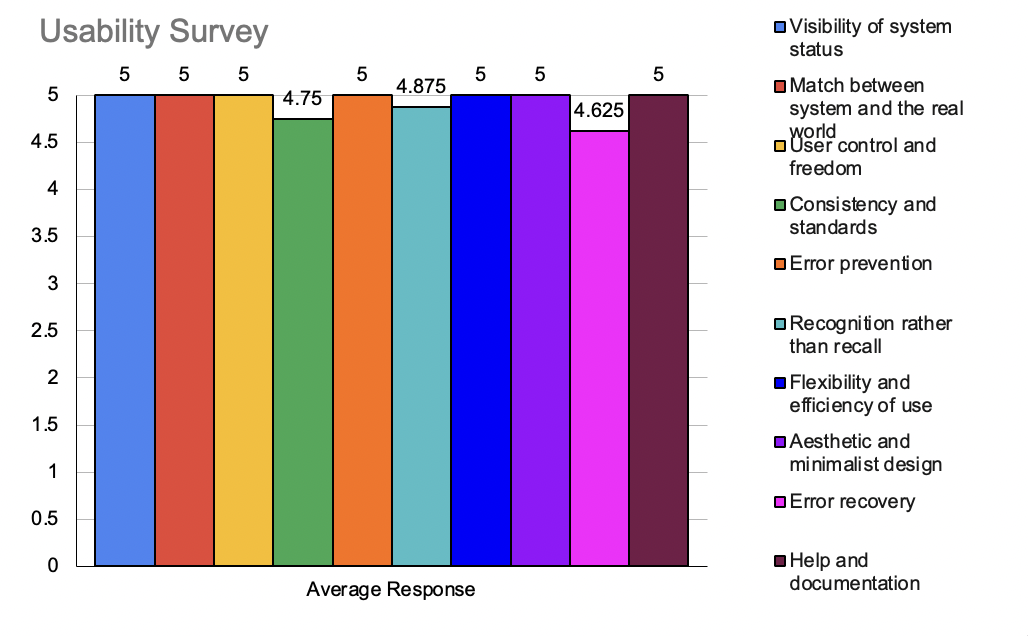
\includegraphics[scale=0.75]{images/UserStudyGraph.png}
    \caption{This graph shows the average response of participants to each of Neilson's 10 Usability Heuristics from the post-study survey carried out as part of the evaluation.}
    \label{fig: UserStudyGraph}
    \end{centering}
\end{figure}

\par 
Most participants strongly agreed that the system was usable and satisfying. For 8 out of the 10 usability
heuristics, participants all strongly agreed that the app entirely met these standards. 
However, 3 of these heuristics, consistency and standards, recognitions rather than recall and error prevention, did not score as highly.
\par 
From this first section of the survey, participants were also able to explain their motivation behind their scorings. 
These open-ended questions were analysed and major themes were identified.
\par 
\textbf{Ease of Use} When giving comments on their answers many participants stated explicitly how they thought the application was 
easy to use, intuitive and clearly laid out, with one participant even stating "Simple to understand for a technophobe like me". 
Other users mentioned that the navigation was clear to follow, with buttons being placed logically so they were easy to find,
and the application used features that were very familiar to typical iOS design and other similar applications. Error messages 
were also stated to be easily identifiable and understandable, users stated that they were 
made clear what the issues were and how they should be solved. Participants also noted that they appreciated the extra help icons 
as they gave more direction to the users on how they should be answering the questions.
This shows that generally users did not find using the application difficult, making for an enjoyable experience.
\par 

\textbf{Issues users had with the application and scorings} For the areas where users did not strongly agree with the heuristic they were
able to give explanations for their answer in the comments. The heuristics for consistency was given 2 agree scores. One
participant stated "I am an adroid user" as their explanation. This could be due to the app mostly following native to iOS design
practices and not being familiar for someone who has experience in only android phones, this could make it more difficult for a user.
The other participant stated as their comment for why they scored consistency as agree "The app used a consistent colour scheme 
throughout and consistent and intuitive navigation options between and within the apps pages and sections. The settings page was 
also made to look similar to the operating systems main settings page. this consistency with other systems made it easy to understand 
its purpose." This does not give a clear indication of why this participant did not score this heuristic as highly as the other 
participants.
\par 
Recognition rather than recall also did not score as highly, with one user scoring this as agree and stating "This was easy to 
understand throughout. On the create note page I scrolled down to understand the full extent of the form and what was required 
of creating a note before completing it." This shows that for this user they were unsure of what would be necessary for them to
reflect before they had looked at the note creation view, meaning that on first viewing of this page the user could potentially 
not be using this note creation to it's full potential. 
\par 
Another participant scored error prevention as neutral, however, this was not stated to be a negative review of the application
as the participant explained "I encountered no errors". This scoring could show that the user did not feel the need to rate this
attribute postively or negatively as they had not witness any errors within the application. 
\par 
\textbf{Future work identified by participants}
\begin{itemize}
    \item In the future, this application could be made cross-platform meaning it would be required to use less iOS design so that 
    it would be suitable for a user with experience with any operating system. Additionally, an android version of this application
    could be made seperately to also fit the needs of more users. 
    \item In the future, more descriptions of the questions users will have to answer and the depth of reflection needed from them 
    could be made more clear in the description of the application. Allowing users to preview what is expected of them before they 
    begin to reflect could help them be more prepared and leas to better reflections.
\end{itemize}
\par 
Following this section of the survey, users then had to answer question relating to their preferences and experience with the application
in general. 
\par 
The survey asked about specific features of the application and recurring themes were identified in each of the comments
for these questions. These questions were useful in targetting the aims of the project to find insight into whether the participants 
felt these were met.
\par 
\textbf{Creating an application to capture reflections on graduate attributes:} The first question asked the users how easy they found reflection. 7 out of 8 participants voted the application as very easy 
to reflect with, with 1 participant voting easy. This shows that for the majority of people, this application was overall 
very useful for users to reflect and provided enough assistance and prompts for the users to reflect on their graduate attributes 
without any issues. However, there is still room for improvement to make this process more seamless for every user.
\par 
\textbf{Allow users to create a note via written or audio form:} All participants stated that they felt the ability to create audio 
recording was useful, with several participants stating that they would be useful for quick and convenient reflections as they are 
less formal. One user stated that "The recording section, in particular, took very 
little time and effort to add to and often saying how you are feeling can make it more memorable, enhancing its usefulness.", showing 
the addition of this audio recording feature assists users in being able to reflect via more than one format, and that there is value
in being able to think out loud about graduate attributes. This ease of reflection could encourage users in the future to carry out 
more casual and frequent reflection. 
\par 
\textbf{Create a usable application:} When asked if users were able to quickly create a note, all participants voted yes. Users stated that
it was intutively designed and easy to just fill in the boxes. One user stated that the questions and prompts helped to break down
their thoughts easily. This shows that the design of the application and the use of the CBT line of questioning and prompts helps
the user to quickly be able make notes based on meaningful reflections. 
\par 
When asked if users would continue to use this application, all participants voted yes. In the comments for this question many participants
noted the ways they felt an application like this would be useful for them in the future. Two participants noted that this application
could be useful for future employment by helping you list the skills you have used that would be crucial to the workplace and help to 
develop their CV, with another participant also stating that it would help them to "see the skills I have developed outside of the 
basics of my degree focus". This shows that participants have identified the key uses for this application and how reflecting on and 
developing these skills is crucial to assist them in their future workplace. Another participant also noted other ways that this app could 
be useful stating "Reflection on what you are able to do and how you feel can be helpful for mental health and also inspire you in 
what you are currently doing", suggesting the application could be used in the future for further benefits than just to employability.
\par 
The majority of users also felt that the statistics page was also useful, with 1 participants stating "Stats aren't my strong point". 
Participants found this would assist in helping them focus on what skills the need to focus on and develop further, with one 
participant noting that it could be encouraging to see what skills have already been developed. This further extends the use cases of the 
application, allowing them to reflect more efficiently as they would be able to see the areas that are weaker. 
\par 
\textbf{Aid reflection:} When asked if participant felt there was enough assistance to aid reflection, all 8 participants voted 
yes. Participants specifically stated that the helper buttons were very useful and they appreciated the additional information to
prompt their reflections, as well as showing how they application was meant to be used. One participant specifically stated 
"I found the prompts helped me to think in a deeper way about the situation I was describing, it gave me time to think about 
my emotions/reactions." This shows that the application meets the needs of users to help them reflect in a more meaningful way.
This reflection would be useful in the future for users to develop their graduate skills further.
\par 

\textbf{Future work identified by participants}
\begin{itemize}
    \item Filtering the notes by clicking on one of the skill categories on the skill cards.
    \item Ability to set goals for number of reflections on a skill and receiving milestone achievements when these are met.
\end{itemize}

\subsection{Limitations}
One major limitation of this evaluation was that it could not have been conducted in person due to the COVID-19 pandemic. Future work
would be recommended to conduct interviews with particpants as this would allow for the interviewer to enquire further and follow-up
on the responses that the participants give. This would allows for further insight into what the participants think about their 
experience with the application.

\section{Overall}
\subsection{Verification of functional requirements}
\subsection{Verification of non-functional requirements}

\section{UI Tests}

In the future the application would require extensive UI and Unit testing to be released for general use by the public, however, due
to the aims of my project only one UI test was created to give a proof of concept idea for the tests that should be created for future
work. The UI feature that has been tested is the users ability to create and save a written note. This was chosen as this is the 
basic necessary requirement for the application to run functionally. 


% \par 
% If you visualise, follow the basic rules, as illustrated in Figure \ref{fig:boxplot}:
% \par 
% See the file \texttt{guide\_to\_visualising.pdf} for further information and guidance.
% \begin{figure}
%     \centering
%     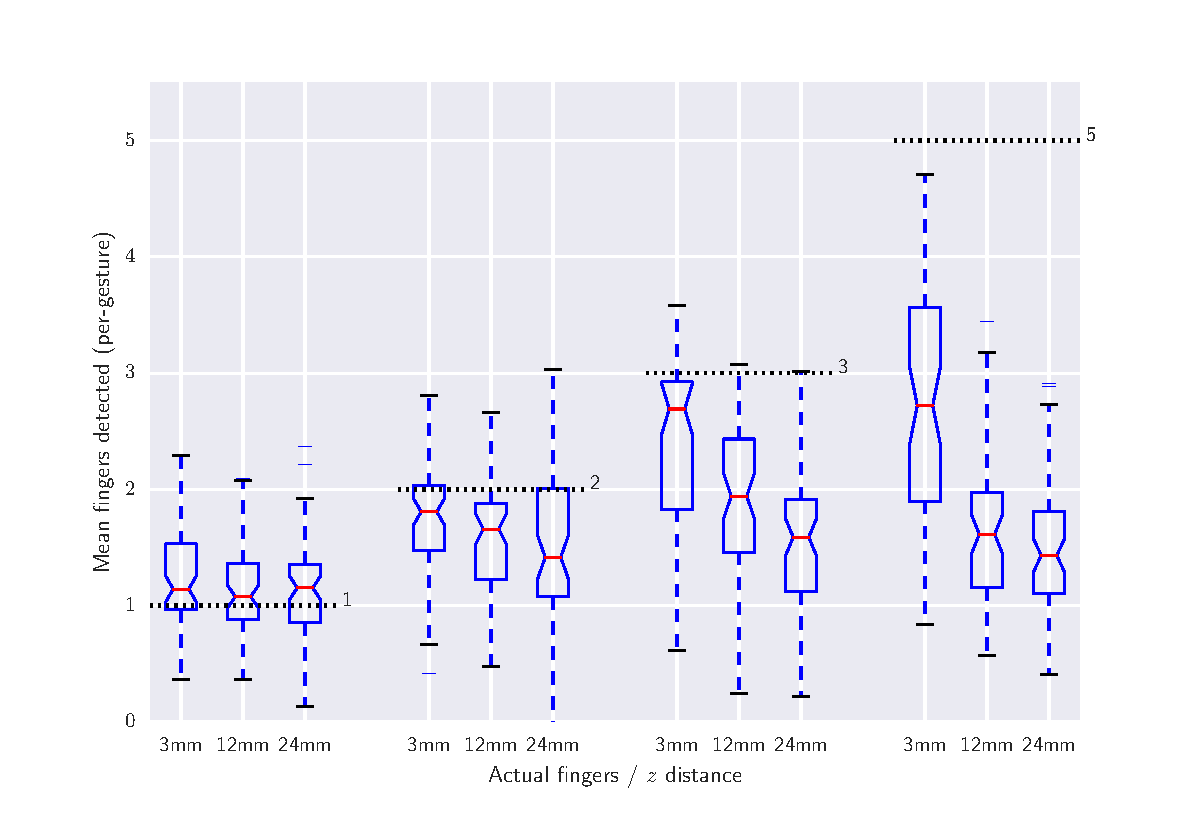
\includegraphics[width=1.0\linewidth]{images/boxplot_finger_distance.pdf}    

%     \caption{Average number of fingers detected by the touch sensor at different heights above the surface, averaged over all gestures. Dashed lines indicate
%     the true number of fingers present. The Box plots include bootstrapped uncertainty notches for the median. It is clear that the device is biased toward 
%     undercounting fingers, particularly at higher $z$ distances.
%     }

%     % use the notation fig:name to cross reference a figure
%     \label{fig:boxplot} 
% \end{figure}


%==================================================================================================================================
\chapter{Conclusion}  

\section{Summary}

Graduate attributes are all the abilities developed by students during their time in university that increase their employability, allows them to 
integrate better into the workplace and creates a better environment within teams. However, there these have been found to be lacking in graduates entering the workplace. This project looked at building an iOS mobile application to capture and encourage reflections on graduate attributes. 

Research was conducted into finding a novel way to encourage reflections through the use of Cognitive Behavioural Therapy (CBT) to explore how the use of this app, with the integration of Cognitive Behavioural Therapy (CBT) techniques, could increase the levels of reflection within students. 

A case study was carried out to asnwer the question: Does CBT benefit reflection by students on their graduate skills? This case study found that students were able to reach higher levels of reflection more frequently than with non-guiding job interview style questions. This gave an indication that this framework has the potential to assist in students development of these skills, as deeper and more meaningful reflection will benefit students in their awareness of these skills. 

The application created, GradRefelct, allows users to capture thier reflection through either written or audio form. Users were given the option of both written and auio format to allow them the oppurtunity to choose whether the wanted to reflect in depth, or the convenience of creating free-form audio recording. It provides a framework using CBT techniques to encourage users to reach all stages of reflection, and provide the neccesary support and instructions to allow them to reflect effectively. The app gives the user detailed descriptions of each skill they are expected to develop and descriptions of how the application is intended to be used. This makes it clear to the user what is expected of them when using this application and, again, gives them clear instructions to allow them to reflect in a beneficial way. GradReflect also gives users insight into their own reflections, providings statistics based on their written notes. It details to users how many notes have been written, their average lengths overall and for each skill, as well as their average emotional responses to skills. This is intended to give users insight into what skills require further development and reflection. The application also provides notifications to encourage the user to reflect regularly. 

GradReflect was evaluated using monitored and survey-based user evaluations. It was found that GradReflect was easy to use, assited their reflection and that they would continue to use this application in the future, with some participants stating various ways they could see it benefitting them. From these results it was clear that an application such as this has the potential to be beneficial for students in developing their graduate skills.


\section{Future Work}

From the case study, implementation and evaluation, there are a number of avenues for future exploration of this topic, as well as changes that could have been made to improve the application. 

The case study conducted at the beginning of the project could be extended into a full experiment where participants answer reflective questions using the CBT framework for an extended period of time. Comparisons between the level of graduate skills before and after the experiment could be used to determine the long-term effects that this proposed method of reflection could have on students. 

The evaluations needed to be conducted in a controlled environment over video conferencing, and so it is possible that some of the participants behaviours were not representative of how they would interact with the application if the app was actually deployed onto their device. Due to this, a reasonable next would be to deploy this application in the future and examine how users would interact in person. It could then also be examined where users skills improve if given access to this application over an extended period of time.

During these evaluations, users presented several ways they would want to see the application itself improved. As well as these improvements from users, there were potential improvements identified personally.

\begin{itemize}
    \item Allow users to delete a note from within a note review view.
    \item The emotion slider could allow users to click where they want the slider to go, as well as being able to drag.
    \item Make the button to delete notes clearer to the users, make it red with a 'delete notes' label next to it, include in the app description that users are able to both click the edit button, and swipe in the typical gesture iOS apps are able to do.
    \item Filtering the notes by clicking on one of the skill categories on the skill cards.
    \item Ability to set goals for number of reflections on a skill and receiving milestone achievements when these are met.
    \item A tab bar could be used to navigate through the application instead of a home page directing to each section.
    \item 
\end{itemize}

If the application were to be deployed to iOS users with an Apple Developer License, futher developments would need to be made such as the extension of notification to fire weekly, and further UI and unite testing to be developed. 


\section{Reflection}

Overall, this project has taught me a great deal in terms of individually organising and carrying out a large-scale piece of work. It was a useful learning oppurtunity, particularly in learning a new language and beginning to use it quickly. The ability to learn a new language and frameworks, and apply these in a solo project has greatly improved my confidence and technical skills. It has highlighted the importance of good project management when working under time contraints. 
The research into different methodologies to encourage reflection and the benefits reflection can have on a student or person, were particularly insightful and these practices will be taken into my future projects and with me into the workplace. Through this project, I feel I have personally developed the key graduate attributes that have been discussed in this paper.


%==================================================================================================================================
%
% 
%==================================================================================================================================
%  APPENDICES  

\begin{appendices}

\chapter{Appendices}

Typical inclusions in the appendices are:

\begin{itemize}
\item
  Copies of ethics approvals (required if obtained)
\item
  Copies of questionnaires etc. used to gather data from subjects.
\item
  Extensive tables or figures that are too bulky to fit in the main body of
  the report, particularly ones that are repetitive and summarised in the body.

\item Outline of the source code (e.g. directory structure), or other architecture documentation like class diagrams.

\item User manuals, and any guides to starting/running the software.

\end{itemize}

\textbf{Don't include your source code in the appendices}. It will be
submitted separately.

\end{appendices}

%==================================================================================================================================
%   BIBLIOGRAPHY   

% The bibliography style is abbrvnat
% The bibliography always appears last, after the appendices.

\bibliographystyle{abbrvnat}

\bibliography{l4proj}

\end{document}
